%
% LaTeX template for prepartion of submissions to PLDI'15
%
% Requires temporary version of sigplanconf style file provided on
% PLDI'15 web site.
%
\documentclass[pldi]{sigplanconf-pldi15}

%
% the following standard packages may be helpful, but are not required
%
\usepackage{SIunits}            % typset units correctly
\usepackage{courier}            % standard fixed width font
\usepackage[scaled]{helvet} % see www.ctan.org/get/macros/latex/required/psnfss/psnfss2e.pdf
\usepackage{url}                  % format URLs
\usepackage{listings}          % format code
\usepackage{enumitem}      % adjust spacing in enums
\usepackage[linesnumbered,ruled]{algorithm2e}
\usepackage{algpseudocode}
\usepackage{graphicx}
\usepackage{amsthm}
%\usepackage{setspace}
\usepackage[colorlinks=true,allcolors=blue,breaklinks,draft=false]{hyperref}   % hyperlinks, including DOIs and URLs in bibliography
% known bug: http://tex.stackexchange.com/questions/1522/pdfendlink-ended-up-in-different-nesting-level-than-pdfstartlink
\newcommand{\doi}[1]{doi:~\href{http://dx.doi.org/#1}{\Hurl{#1}}}   % print a hyperlinked DOI
%\doublespacing

\newtheorem{lemma}{Lemma}
\newtheorem{theorem}{Theorem}
\newtheorem{definition}{Definition}

\begin{document}

%
% any author declaration will be ignored  when using 'plid' option (for double blind review)
%

% TODO CAMREADY: Don't forget to run e.g. s/\\quicksand /\\quicksand~/
\newcommand\landslide{\textsc{Landslide}}
\newcommand\quicksand{\textsc{Quicksand}}
\newcommand\simics{\textsc{Simics}}
\newcommand{\sect}[1]{\S #1}
\newcommand\hilight[2]{\color{#1}#2\color{black}}
\definecolor{orange}{RGB}{192,96,0}
\definecolor{olivegreen}{RGB}{0,127,0}
\definecolor{brickred}{RGB}{192,0,0}
\definecolor{commentblue}{RGB}{0,0,192}

\newcommand\numthrlibs{79}
\newcommand\numpintoses{78} % 'di' is basecode. durr
\newcommand\numstudence{157} % total pintoses plus p2s

\title{Stateless Model Checking with Data-Race Preemption Points}
\authorinfo{Ben Blum}{Carnegie Mellon University}{bblum@cs.cmu.edu}
\authorinfo{Garth Gibson}{Carnegie Mellon University}{garth@cs.cmu.edu}

\maketitle
\begin{abstract}
Stateless model checking is a powerful technique for testing concurrent programs,
but suffers from exponential state space explosion when the test input parameters are too large.
Several reduction techniques can mitigate this explosion,
but even after pruning equivalent interleavings, the state space size
%for a fixed set of preemption points
is often intractable.
Most prior tools are limited to preempting only on synchronization APIs,
which reduces the space further, but can miss unsynchronized thread communication bugs.
%
Data race detection, another concurrency testing approach, focuses on suspicious memory access pairs during a single test execution.
It avoids concerns of state space size, but is prone to false positives:
spurious reports of access pairs that cannot be reordered to produce a bug.

We present an {\em Iterative Deepening} framework for stateless model checking,
which manages the exploration of many state spaces using different preemption points.
It uses state space estimation to prioritize jobs most likely to complete in a fixed CPU budget,
and it incorporates data-race analysis to add new preemption points on the fly.
Preempting threads during a data race's instructions
%These preemption points allow us to check whether each data-race can produce an observable failure, and
can automatically classify the race as buggy or benign,
and uncovers new bugs not reachable by prior model checkers.
%
It also enables full verification of all possible schedules when every data race is verified as benign within the CPU budget.
In our evaluation, Iterative Deepening
%with data-race preemption points
found 1.8x as many bugs and verified 4.3x as many tests compared to stateless model checking without data-race preemption points.
%Our evaluation shows this technique is
%more effective than single-state-space model checking
%%both at finding more bugs and at completing more state spaces when no bug exists.
%both at finding the same bugs faster and at finding new bugs entirely.

\end{abstract}

%%%%%%%%%%%%%%%%%%%%%%%%%%%%%%%%%%%%%%%%%%%%%%%%%%%%%%%%%%%%%%%%%%%%%%%%%%%%%%%%

\section{Introduction}

% blah blah trite opening sentence
%As parallelism becomes ever more important for achieving high performance in modern-day programs,
%so too do advanced concurrency testing techniques become important for verifying the correctness of those programs.
Concurrency bugs are notoriously hard to find and reproduce because they only appear in specific thread interleavings, which arise at random during normal program execution.
{\em Stateless model checking} \cite{verisoft} offers a method for finding such bugs,
or verifying their absence,
%by systematically executing a program along as many distinct interleavings as possible,
by forcing a program to execute each distinct interleaving,
capturing and controlling this nondeterminism using a finite state space.
Unfortunately, these state spaces explode exponentially in the size of the input program.
Reduction techniques such as Dynamic Partial Order Reduction \cite{dpor} and Maximal Causality Reduction \cite{mcr} expand the limits of feasible test completion,
and search ordering strategies such as Iterative Context Bounding \cite{chess-icb} allow bugs to be found sooner in a given exploration should they exist.

% Can I even make a claim this broad to begin with?
However, all stateless model checkers to date are bound by a fixed set of {\em preemption points}: code locations that define the granularity at which threads interleave.
% TODO: You repeat the following 1.5 sentence in the related work section; maybe you can eliminate this redundancy to save space?
For example, \textsc{CHESS} \cite{chess} preempts only on synchronization operations and library calls, which can miss lock-free shared memory races.
It provides an additional data-race analysis to report any violations of this model;
however, data-race analyses are prone to report false positives
%and benign races
which require annotations or imprecise heuristics to suppress \cite{racerx,tsan,datacollider}.
%
On the other hand, SPIN \cite{spin}
is able to preempt threads around any shared memory access. Such fine granularity would automatically check if each data race is a real bug, but makes full state space completion intractable for even modestly-sized tests.
%
Configuring a model checker is a tradeoff between schedule coverage and feasibility of completion.
This work shows how to avoid making that tradeoff decision in advance.

% TODO: ttuttle says this is too much of a jump -- that exactly what "subsets" means is not well defined (i.e, lock vs unlock, while NOT addressing the within/without_function problem)

We present \quicksand, a framework for {\em Iterative Deepening} of preemption points during stateless model checking.
Named after the analogous technique in chess AI \cite{iterative-deepening-chess-ai}, our approach likewise makes progressively deeper searches of the state space until a given CPU budget is exhausted.
Rather than attempting to search a single state space with every available preemption point enabled (e.g., preempting on every pthread API call),
\quicksand~tests many different state spaces corresponding to subsets of those points, managing a model checker instance to explore each one.
It estimates the size of each state space to decide when long-running instances should be suspended, and dynamically generates new state spaces based on data race analysis.
%In fact, if given enough time to fully test all discovered data-race preemption points,
%Iterative Deepening provides a full verification of all thread schedules that could arise from preempting anywhere.
In fact, Iterative Deepening is fully general:
we prove that if it completes all state spaces resulting from data-race preemption points,
that serves as a total verification of all possible thread interleavings of the given test program.

We evaluate \quicksand~by testing \numstudence~student thread libraries and kernels from the undergraduate OS classes at Carnegie Mellon, Berkeley, and the University of Chicago.
\quicksand~finds more bugs than the conventional stateless model checking approach given the same CPU budget,
% joshua wants me to say "conventional approachES" here
and furthermore, adding data-race preemption points quickly exposes bugs missed by even the ``maximal'' state space of the conventional approach.

This paper's contributions are as follows:
\begin{enumerate}
	\item Iterative Deepening, a new technique for combining data-race analysis with stateless model checking, and \quicksand, an open-source implementation of the technique;
	\item A proof of convergence, which shows that should it be possible in the given CPU budget,
		fully testing every discovered data-race preemption point is equivalent to testing all possible thread schedules;
	\item A new tactic for eliminating one class of false-positive data races,
		which cannot soundly be used in a single-pass analysis,
		but which we prove correct when used with Iterative Deepening;
		%, unsound in single-pass analysis but which we prove sound when used with Iterative Deepening;
	%\item Techniques for detecting and flattening cyclic state spaces resulting from ad-hoc while-loop synchronization % TODO: is there actually room for this in the paper?
	\item A large evaluation in which \quicksand~compares favorably to stand-alone data-race detection and stateless model checking approaches.
\end{enumerate}

The remainder of the paper is organized as follows.
\sect{\ref{sec:design}} discusses the background and design of Iterative Deepening, including our proof of convergence,
\sect{\ref{sec:implementation}} explains \quicksand's approach to implementing it, including our new false-positive data-race tactic,
\sect{\ref{sec:eval}} presents our evaluation,
\sect{\ref{sec:future}} discusses limitations and future work,
\sect{\ref{sec:related}} surveys the related work,
and \sect{\ref{sec:conclusion}} concludes.

\section{Background}
\label{sec:overview}

We review the background in stateless model checking and data-race analysis using the example program in Figure~\ref{fig:example}.

\begin{figure}[t]
	\small
\begin{tabular}{rll}
	& \multicolumn{2}{c}{\texttt{int x = 0; mutex\_t mx;}} \\
	& {\bf Thread 1} & {\bf Thread 2} \\
	1 & \texttt{\hilight{orange}{mutex\_lock(\&mx);}} & \\
	2 & \texttt{int tmp = x;} &\\
	3 & & \texttt{atomic\_xadd(\&x, 1);} \\
	4 & & \texttt{\hilight{olivegreen}{yield();}} \\
	5 & & \texttt{atomic\_xadd(\&x, 1);} \\
	6 & \texttt{x = tmp + 1;} & \\
	7 & \texttt{\hilight{commentblue}{mutex\_unlock(\&mx);}} & \\
	8 & & \texttt{assert(x >= 2);} \\
	%1 & \texttt{\hilight{brickred}{x->foo = ...;}} & \\
	%2 & \texttt{\hilight{olivegreen}{free}(x);} \\
	%3 & & \texttt{\hilight{commentblue}{// x's memory recycled}} \\
	%4 & & \texttt{y~=~\hilight{olivegreen}{malloc}(sizeof *y);} \\
	%5 & & \texttt{\hilight{commentblue}{// ...initialize...}}\\
	%6 & & \texttt{publish(y);} \\
	%7 & & \texttt{\hilight{brickred}{y->bar = ...;}} \\
\end{tabular}
\caption{Example program with a data-race bug. In this interleaving, the assertion on line 8 will fail. Two data-race preemptions are required to expose the bug: one just before thread 1's line 6, and one just before thread 2's line 8.}
\label{fig:example}
\end{figure}

\subsection{Stateless Model Checking}

Stateless model checking \cite{verisoft} is a testing technique for systematically exploring the possible thread interleavings of a concurrent program.
A stateless model checker executes the program repeatedly, each time according to a new thread interleaving, until the state space (or the CPU budget) is exhausted.
Rather than identifying suspicious conditions which may include false alarms, the approach of many static analyses \cite{racerx,coverity},
stateless model checkers focus on concrete observable failures such as assertions, deadlocks, and segfaults.

\begin{figure}[t]
	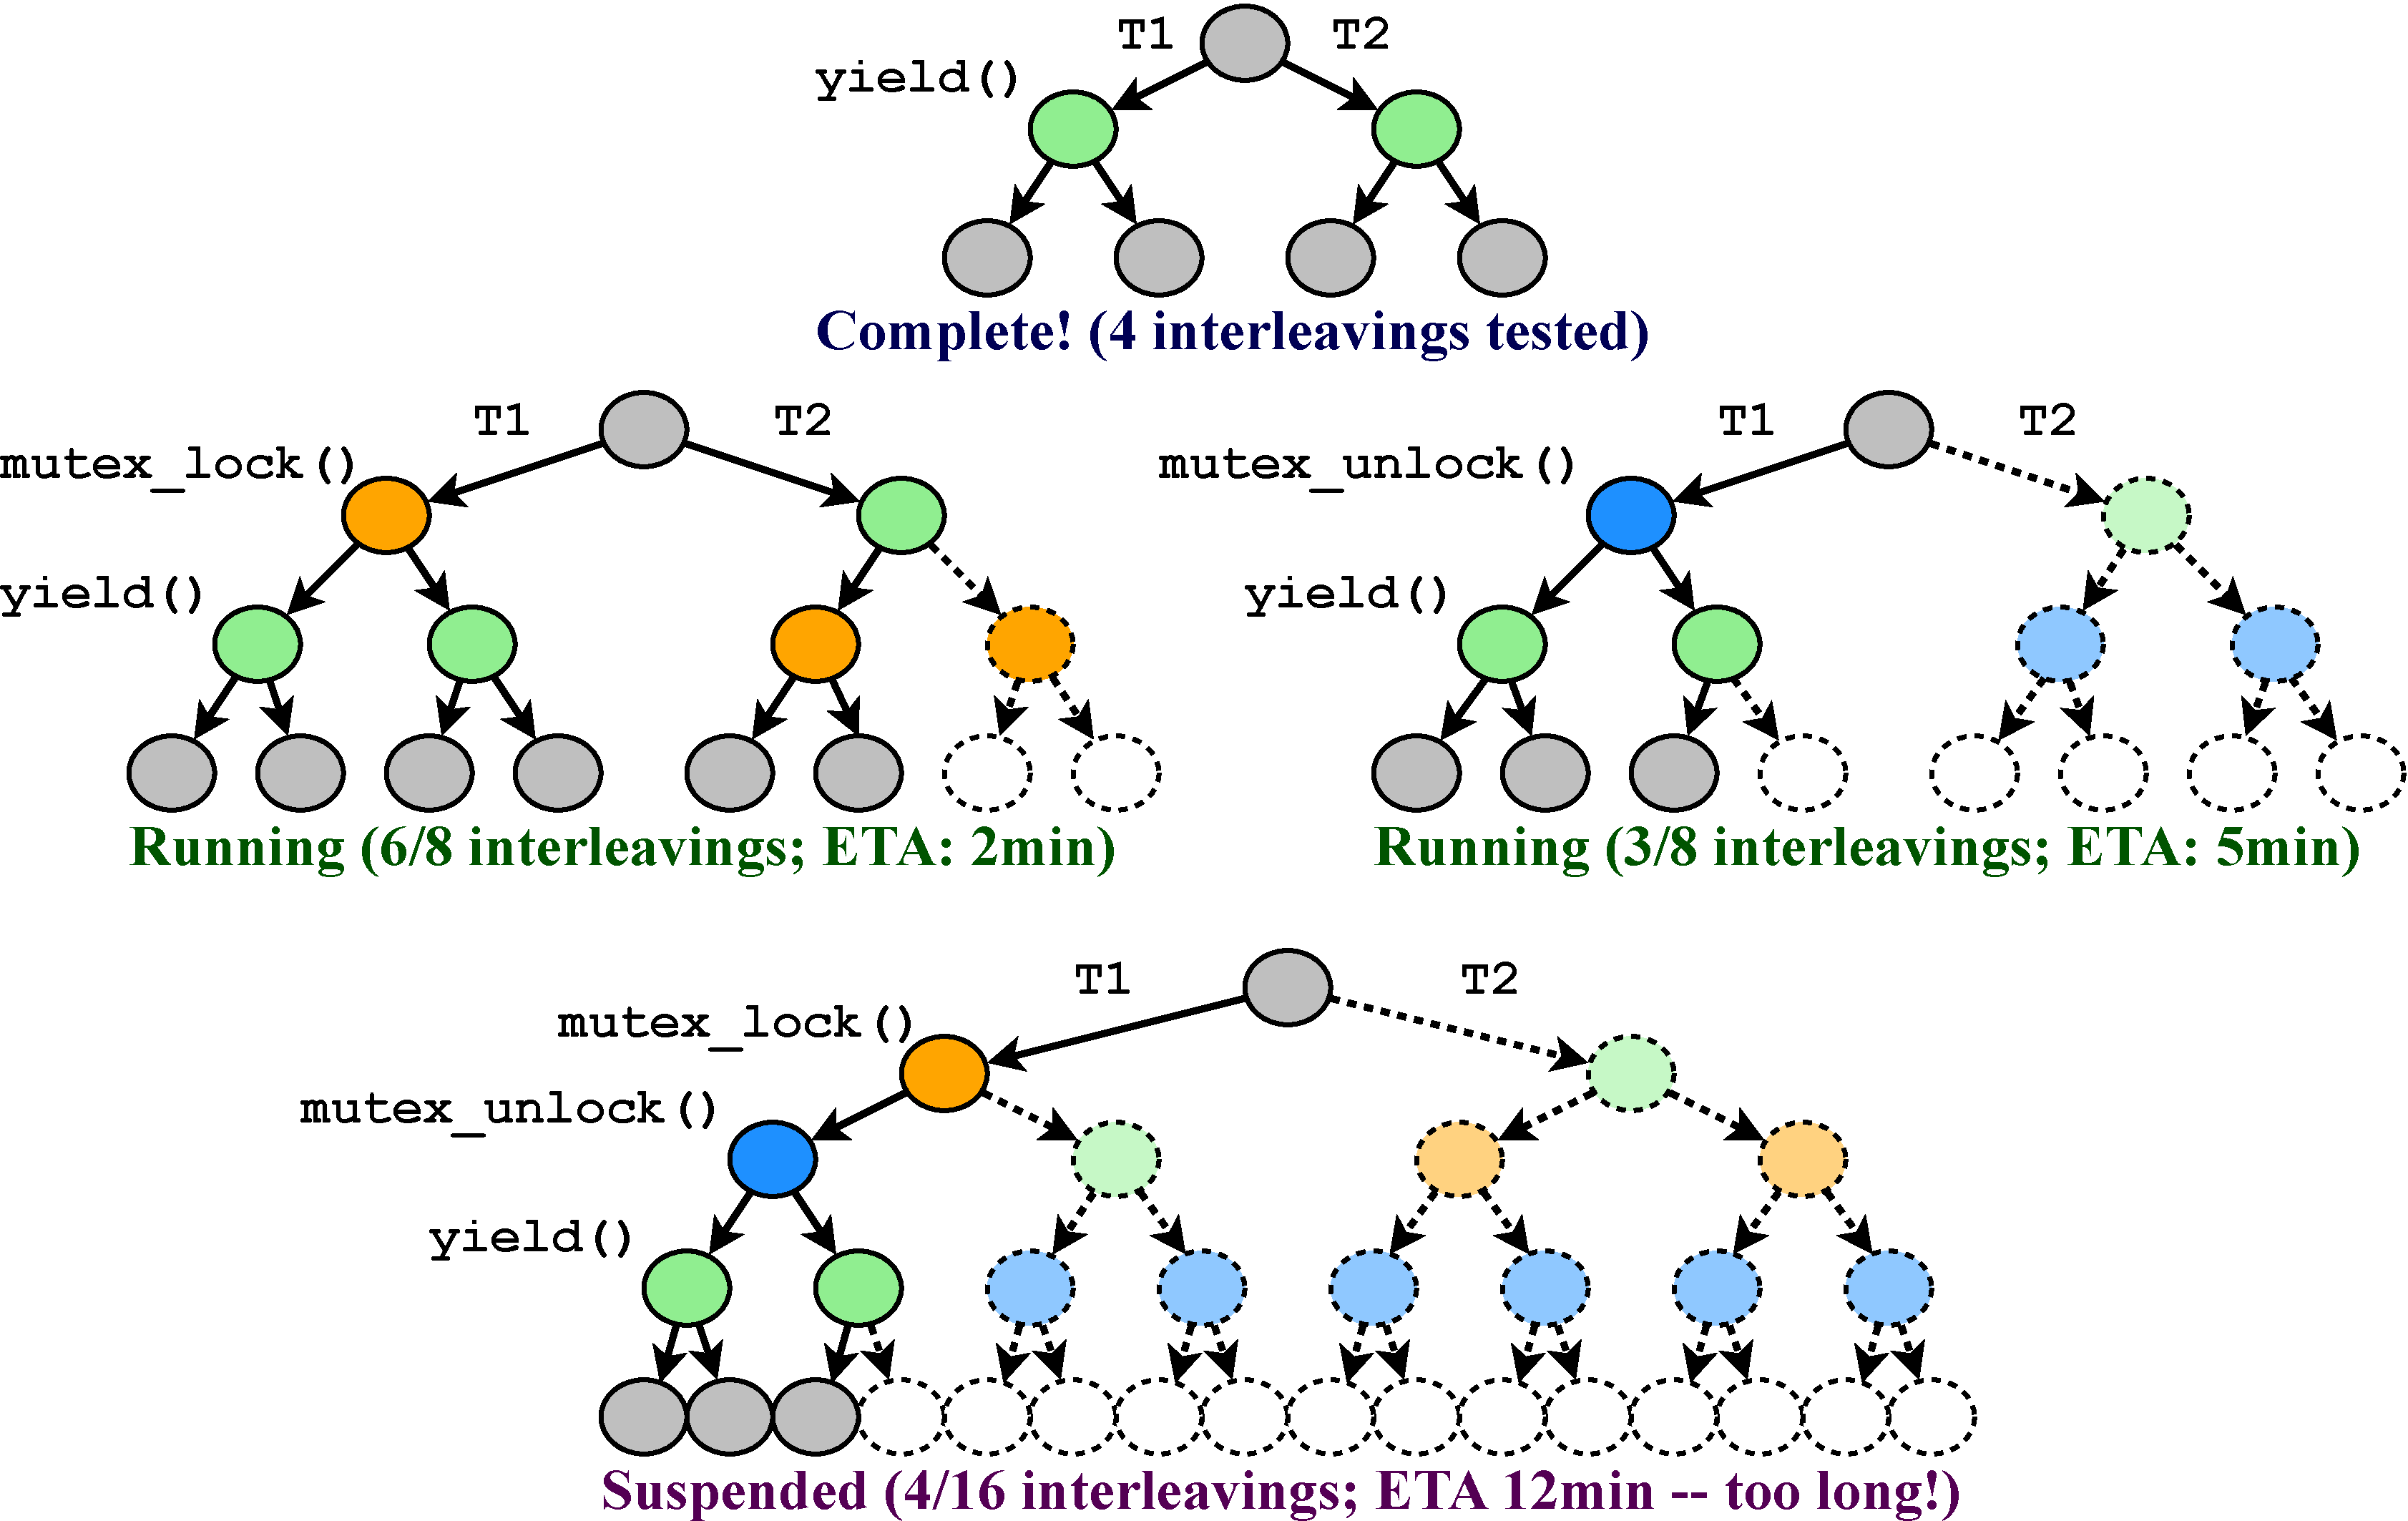
\includegraphics[width=0.48\textwidth]{trees-v2-squashed.pdf}
	\caption{Iterative Deepening example.
		The minimal state space (top) includes only voluntary thread switches, such as {\tt yield()}. %or {\tt cond\_wait()}.
		Multiple further tests can be run: preempting on calls to {\tt mutex\_lock} alone (left), {\tt mutex\_unlock} alone (right), or both together (bottom).
Each option increases the state space size unpredictably, so multiple state spaces should be tested in parallel.
Estimation techniques~\cite{estimation} inform which state spaces to prioritize.
}
	\label{fig:id}
\end{figure}

The checker defins the granularity of thread interleavings by which {\em preemption points} it uses to switch threads.
Most model checkers \cite{chess,dbug-ssv} choose synchronization/thread library API boundaries for these points;
in our example program, these would be lines 1, 4, and 7.
Figure~\ref{fig:id} shows several possible resulting state spaces.
The approach of prior work is to enable all preemption points simultaneously, i.e., to test only the bottom state space.

To mitigate the exponential explosion,
Dynamic Partial Order Reduction \cite{dpor} identifies equivalent execution sequences according to Mazurkiewicz trace theory \cite{mazurkiewicz},
and tests at least one execution from each equivalence class.
Intuitively, if two thread transitions between preemption points do not conflict on any shared resource access, reordering them produces an equivalent interleaving.
Nevertheless, state spaces are still exponentially-sized in the number of conflicting transitions.

This motivates {\em Iterative Deepening}, our new technique for heuristically adjusting the preemption points at runtime.
Rather than committing to one state space with every available preemption point enabled,
Iterative Deepening searches among different {\em subsets} of the points;
for example, ``preempt on all calls to {\tt mutex\_lock} but not on {\tt mutex\_unlock}''.
Hence, we will test all the state spaces shown in Figure~\ref{fig:id} in parallel,
and decide on-the-fly whether to pursue each test, or to defer it in favour of smaller ones.

\subsection{Data Race Detection}

Data race analysis \cite{eraser} identifies pairs of unsynchronized memory accesses between threads.
Two instructions are said to race if
they both access the same memory address,
at least one is a write,
the threads do not hold the same lock,
and no synchronization enforces the order of the thread transitions.
Data races are not necessarily bugs, but represent suspicious violations of the locking discipline.
In Figure~\ref{fig:example}, lines 3 and 5 each race with 2 and 6, and line 6 races with 8.

Though state-of-the-art MCs preempt only on synchronization events,
many serious concurrency bugs are caused by data races leading to corrupted shared state.
Figure~\ref{fig:example}'s thread interleaving is possible only with {\em data-race preemption points}:
preempting a thread just before an instruction identified as part of a data race.
None of the state spaces in Figure~\ref{fig:id} contain this interleaving,
as none of the mutex/yield preemptions split lines 2 and 6 across different transitions.

Prior work \cite{hybriddatarace} distinguishes between {\em pure happens-before} \cite{lamport-clocks},
in which accesses with a lock release/acquire in between are not considered concurrent,
and {\em limited happens-before},
in which only blocking operations like {\tt cond\_wait} or {\tt join} enforce the order.
Compared to the former, the latter may output false positives, but avoids false negatives \cite{tsan},
which is more appropriate for this work (\sect{\ref{sec:totalverif}}).

\subsection{Terminology}

For the rest of the paper, we will abbreviate {\em preemption point} (PP),
%For the remainder of the paper, we will abbreviate {\em preemption point} (PP),
{\em model checking} (MC),
{\em single-state-space model checking} (SSS-MC), % (i.e., the approach of prior work),
{\em Dynamic Partial Order Reduction} (DPOR), and {\em state space estimate} (ETA).

SSS-MC indicates the approach of prior tools:
the set of PPs is fixed in advance, and the tool commits to testing every interleaving available with those PPs.
%Reduction techniques are often used to skip equivalent interleavings \cite{dpor}, and search-ordering strategies
Many techniques can skip equivalent interleavings or order the search to uncover bugs faster \cite{dpor,demeter,chess-icb,gambit,smc-empirical-study},
but new PPs cannot be added, nor ineffective ones removed, by any dynamic analysis.

Although all data races are undefined behaviour in C and C++ \cite{boehm-memorymodels},
we distinguish between data-race {\em candidates} and data-race {\em bugs}.
Because data-race analysis is prone to false-positives,
we classify unprotected access pairs separately from bugs,
calling such pairs {\em data race candidates}.
Should a future interleaving, preempting during those accesses,
lead to a failure, then we report a {\em data-race bug}.
Otherwise, if the access pair can be reordered, but does not produce a failure under any interleaving, it is a {\em benign data race}.
If they cannot be reordered at all, it is a {\em false positive}.
%TODO: Don't do this, below. Scan paper for uses of 'false positive' where you mean to say 'benign' or 'both'.
%For brevity, we count benign data races as a subset of false positives.

We also identify the {\em minimal} and {\em maximal state space} for each test.
The {\em minimal state space} includes only thread switches arising from normal execution (Figure~\ref{fig:id}, top).
The {\em maximal state space} is the one tested by SSS-MC: all statically-available PPs are enabled (Figure~\ref{fig:id}, bottom).
%However, should new data-race PPs be added during a test, the new maximal state space will be the one including those as well.
%% don't say this ^ -- because when you add dr pps, they add in pairs and there would be multiple maximals, at least until they each get explored and subseuqnetly add a pp of the other of the pair.

\section{Design}
\label{sec:design}

Named after the analogous technique in chess artificial intelligence \cite{iterative-deepening-chess-ai},
Iterative Deepening
%likewise
makes progressively deeper searches of the state space until the CPU budget is exhausted.
In this context, the depth is the number of PPs used.
Hence, our tool \quicksand~schedules multiple MC instances in parallel to simultaneously test many different subsets of the available PPs.
%which we refer to as {\em jobs}.
We refer to each unique set of PPs as a {\em job},
and prioritize them based on number of PPs, ETA, and whether they include data-race PPs,
We rely on state-space estimation \cite{estimation}
to predict which jobs are likely to complete within a reasonable time,
before actually testing a large fraction of interleavings for each.
The overall goal is to decide automatically when to defer testing a state space,
so an inexpert user can provide only their total CPU budget as a test parameter,
and to enable completing appropriately-sized jobs within that budget.
We seek to maximize completed state spaces,
as each one serves as a guarantee that all interleavings possible with its PPs were tested.

Note that Iterative Deepening is a {\em wrapper} algorithm around stateless MC.
A MC tool is still used to test each state space, and other reduction techniques are still applicable.
Moreover, because Iterative Deepening treats the set of preemption points as mutable,
it can add new preemption points reactively based on any runtime analysis.
We focus on run-time data-race detection~\cite{hybriddatarace,tsan,ifrit} as the mechanism for finding new preemption candidates.

%%%%%%%%%%%%%%%%%%%%%%%%%%%%%%%%%%%%%%%%%%%%%%%%%%%%%%%%%%%%%%%%%%%%%%%%%%%%%%%%

\subsection{Initial PP configuration}

Iterative Deepening must be seeded with a set of initial state spaces,
which can be any number of subsets of the statically-available PPs SSS-MC would use.
For completeness (\sect{\ref{sec:totalverif}}), the maximal state space must be included among these.

For testing user-space code, we begin with the four PP sets from Figure~\ref{fig:id}:
$\{yield\}$,
$\{yield,lock\}$,
$\{yield,unlock\}$,
and $\{yield,lock,unlock\}$,
By extension, these also introduce PPs on any other primitives
which use
internal locks,
such as condvars or semaphores.
Preempting on voluntary switches such as {\tt yield} is always necessary to maintain the invariant that only one thread runs between consecutive PPs.
%so the {\tt yield} PP is always implicitly enabled.

For kernel-level testing, we consider interrupt-disabling analogous to locking,
so we also preempt just before a disable-interrupt opcode ({\tt cli}) and just after interrupts are re-enabled ({\tt sti})\footnote{
%(to appropriate the names of the x86 instructions)
During data-race detection, {\tt cli}/{\tt sti} are treated as a single global lock.
%as {\tt cli}'d memory accesses can still race with others that have interrupts on.
Some kernels disable preemption without disabling interrupts,
which can be communicated to the MC using manual annotations. %of that API.
This also assumes uni-processor scheduling; for SMP kernels, replace {\tt cli}/{\tt sti} with spinlocks.}.
\quicksand~is configured to begin with
$\{yield\}$,
$\{yield,lock\}$,
$\{yield,unlock\}$,
$\{yield,cli\}$,
$\{yield,sti\}$,
and $\{yield,lock,$ $unlock,cli,sti\}$.
As a heuristic, we don't test every intermediate subset such as $\{lock,sti\}$,
which could potentially be improved in future work (\sect{\ref{sec:future}}).

%%%%%%%%%%%%%%%%%%%%%%%%%%%%%%%%%%%%%%%%%%%%%%%%%%%%%%%%%%%%%%%%%%%%%%%%%%%%%%%%

\subsection{Choosing the best job}

\newcommand\PendingJobs{\ensuremath{\mathcal{P}}}
\newcommand\SuspendedJobs{\ensuremath{\mathcal{S}}}
\newcommand\GetETA[1]{ETA(#1)}
\newcommand\GetPPSet[1]{PPSet(#1)}
With a limited CPU budget, we must avoid running tests that are likely to be fruitless.
Hence, we separate the available PP sets into a set of {\em suspended} jobs (partially-explored state spaces with high ETAs),
and a set of {\em pending} jobs (untested ones with unknown ETAs).
When the MC reports an ETA too high for some job,
we compare with other pending and suspended jobs to find another one more likely to complete in time.
%
Our method for doing so, listed in Algorithm~\ref{alg:shouldworkblock}, is the heart of Iterative Deepening.
%\footnote{
%Though its worst-case performance is $O(mn)$ in the
%%number of pending and suspended jobs,
%sizes of $\mathcal{P}$ and $\mathcal{S}$,
%in practice the non-constant portion beyond line 4 runs very infrequently
%and is negligible compared to the exponentially-sized state spaces.}.
Its main feature is understanding that if \GetPPSet{$j_1$} $\subset$ \GetPPSet{$j_2$},
and $j_1$ is suspended,
then $j_2$'s state space is guaranteed to be strictly larger, so $j_2$ will take at least as long.
Hence we should avoid testing $j_2$ unless $j_1$ is later resumed and its ETA improves after further execution. %over time.
%reveals that it might finish in time after all.
Similarly, whenever a job finds a bug, we cancel all pending superset jobs, as they would find the same bug.

\begin{algorithm}[t]
	\SetKwInOut{Input}{Input}
	%\textbf{Function} GetBestJob($j_0$, PendingJobs, SuspendedJobs): \\
	\Input{$j_0$, the currently-running job}
	%\Input{$eta$, $j_0$'s predicted completion time}
	\Input{\PendingJobs, the list of pending jobs, sorted by decreasing heuristic priority}
	\Input{\SuspendedJobs, the list of already-suspended jobs, sorted by increasing ETA}
	\If{\GetETA{$j_0$} $<$ HeuristicETAFactor $\times$ TimeLeft()}{
		return $j_0$ // Common case: job is expected to finish.
	}
	\ForEach{job $j_P \in$ \PendingJobs}{
		// Don't run a pending job if a subset of it is already suspended; its ETA would be at least as bad. \\
		\If {$\forall j_S \in$ \SuspendedJobs, \GetPPSet{$j_S$} $\not\subset$ \GetPPSet{$j_P$}}{
			return $j_P$
		}
	}
	%// no pending jobs; maybe resume a suspended job \\
	\ForEach{job $j_S \in$ \SuspendedJobs}{
		\If{\GetPPSet{$j_0$} $\not\subset$ \GetPPSet{$j_S$}
			$\land$
			\GetETA{$j_0$} $>$ \GetETA{$j_S$}}{
			// If a subset of $j_S$ is also suspended, don't run the larger one first. \\
			\If{$\forall j_{S2} \in$ \SuspendedJobs, \GetPPSet{$j_{S2}$} $\not\subset$ \GetPPSet{$j_S$}}{
				return $j_S$
			}
		}
	}
	return $j_0$ // \GetETA{$j_0$} was bad, but no other $j$ was better.
	\caption{Suspending exploration of a state space in favour of a potentially smaller one.}
	\label{alg:shouldworkblock}
\end{algorithm}

%
We also account for the inherent inaccuracy of ETA estimates.
Line 1 heuristically scales up the time remaining to avoid suspending jobs too aggressively
in case their ETAs are actually overestimated.
Lines 12-14 account for the
%bizarre
possibility that among two suspended jobs,
%given two jobs,
%%$j_1,j_2$,
\GetPPSet{$j_1$} $\subset$ \GetPPSet{$j_2$}
but
\GetETA{$j_1$} $>$ \GetETA{$j_2$}.
This can arise because estimates tend to get more accurate over time,
and $j_1$ perhaps ran much longer before suspending.
% In such scenarios,
We heuristically assume the smaller job's ETA is more accurate
to avoid repeatedly resuming larger jobs briefly while their ETAs only become worse
(it lets us avoid thrashing in \quicksand).

%%%%%%%%%%%%%%%%%%%%%%%%%%%%%%%%%%%%%%%%%%%%%%%%%%%%%%%%%%%%%%%%%%%%%%%%%%%%%%%%

\subsection{Data-race preemption points}
\label{sec:classifying}

During stateless MC, runtime data-race detection may find data-race candidates that we wish to investigate further.
Because data races indicate access pairs that can interleave at instruction granularity,
it is logical to re-execute the test and issue preemptions just before those instructions to test alternate thread interleavings~\cite{racefuzzer,portend}.

\newcommand\AllJobs{\ensuremath{\mathcal{J}}}
\begin{algorithm}[t]
	\SetKwInOut{Input}{Input}
	\Input{$j_0$, the currently-running job}
	\Input{\AllJobs, the set of all existing (or completed) jobs}
	\Input{$\alpha$, an instruction reported by the MC as part of a racing access pair}
	\If{$\forall j \in \AllJobs,$
	\GetPPSet{$j_0$} $\cup$ $\alpha$
	$\not\subseteq$
	\GetPPSet{$j$}
	}{
		AddNewJob(\GetPPSet{$j_0$} $\cup$ $\alpha$, HeuristicPriority($\alpha$)) \\
	}
	\If{$\forall j \in \AllJobs,$ \GetPPSet{$j$} $\neq \{\alpha\}$}{
		AddNewJob($\{yield, \alpha\}$, HeuristicPriority($\alpha$))
	}
	\caption{Adding new jobs with data-race PPs.}
	\label{alg:handledatarace}
\end{algorithm}

With Iterative Deepening, this is a simple matter of creating a new state space with an additional PP enabled on the racing instructions by each thread, as shown in Algorithm~\ref{alg:handledatarace}.
We call these {\em data-race PPs}.
Note that even though a data race may involve two different instructions, $\alpha$ and $\beta$, we add new state spaces with only one new PP at a time.
Rather than adding a single large state space, %configured to preempt on both involved instructions,
i.e., $AB =$ \GetPPSet{$j_0$} $\cup$ $\alpha$ $\cup$ $\beta$,
we prefer to add multiple smaller jobs which have a higher chance of completing in time, i.e.,
$A =$ \GetPPSet{$j_0$} $\cup$ $\alpha$ and
$B =$ \GetPPSet{$j_0$} $\cup$ $\beta$.
If $A$ and $B$ are bug-free, they will in turn add $AB$ later.
%We take care to avoid duplicating any superset state spaces with PPs on multiple data races.
The condition on line 1 ensures that we avoid duplicating any state spaces with multiple data-race PPs;
for example, $AB$ is reachable by multiple paths through its different subsets, but should be added only once.

Furthermore, we do not always strictly increase the number of PPs when we find a new data race.
%When \quicksand~receives a data race report, it adds two new jobs to its workqueue:
For each instruction involved in a data race, \quicksand~adds two new jobs:
a ``small'' job to preempt on that instruction only (line 5),
and a ``big'' job to preempt on that instruction as well as each PP used by the reporting job (line 2).
%
Hence,
%together with the logic in \sect{\ref{sec:classifying}},
each {\em pair} of racing accesses will spawn four new jobs, as shown in Figure~\ref{fig:new-dr-jobs}.
%
The rationale of spawning multiple jobs is that we don't know in advance which will be most fruitful: %which will be most fruitful is not known in advance:
while the big job risks not completing in time,
the small job risks missing the data race entirely if the original PPs were required to expose it.
% TODO CAMREADY: Put numbers here.
In practice, we observed some bugs found quickly by these small jobs, and other bugs missed by the small jobs found eventually by the big jobs.
%which motivates the need for Iterative Deepening to prioritize the jobs at runtime.
This phenomenon motivates Iterative Deepening to prioritize the jobs at run-time.

\begin{figure}[t]
	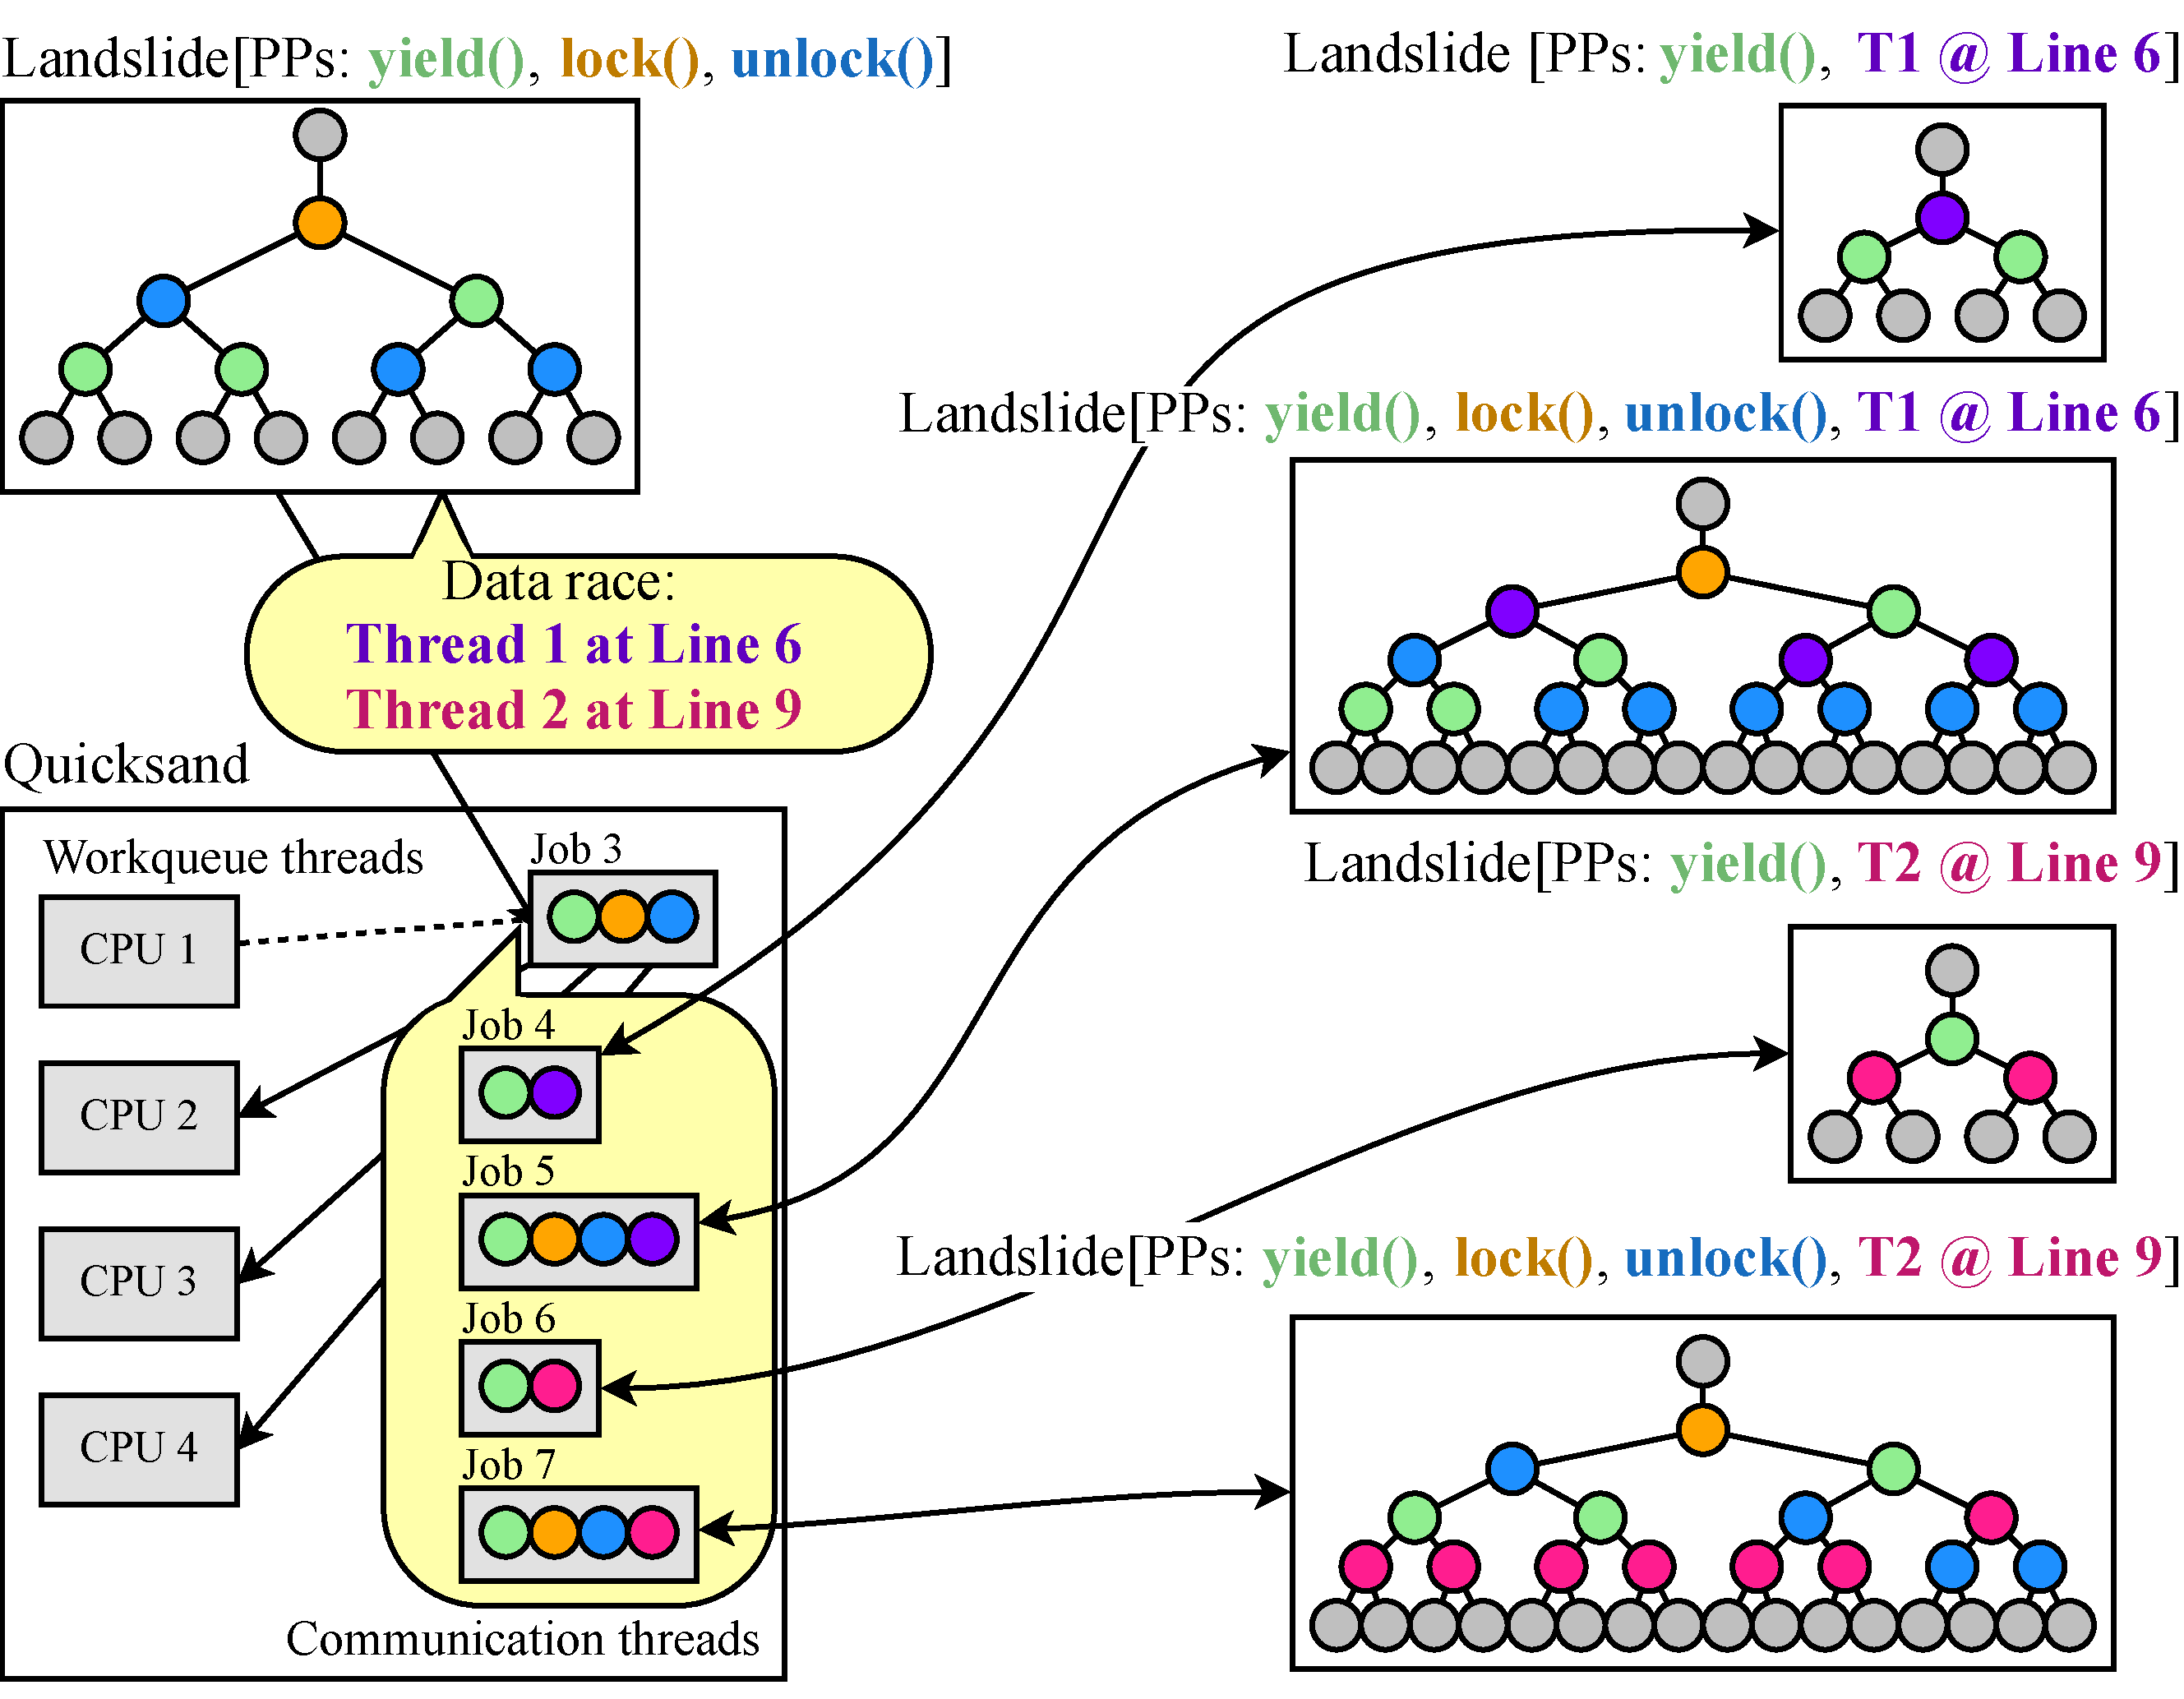
\includegraphics[width=0.48\textwidth]{dr-jobs-v2.pdf}
	\caption{\quicksand~manages the exploration of multiple state spaces, communicating with each MC instance to receive ETAs, data race candidates, and bug reports.
		When an access pair is reported as a data race candidate, we generate a new PP for each access, and add new jobs corresponding to different combinations of those with the existing PPs.}
	\label{fig:new-dr-jobs}
\end{figure}

The new state spaces may expose a failure, in which case we report a data-race bug,
or complete successfully, indicating a benign or false-positive data race.
They may also uncover a new data-race candidate entirely, %in some alternate interleaving,
in which case we may iteratively advance to a superset state space containing PPs for both racing access pairs.
%Because Iterative Deepening is
Being constrained by a CPU budget,
we may time out before completing a data race's associated state space,
in which case we report a potential false positive that the user must handle (\sect{\ref{sec:future}}).

%When \landslide~detects a data race, it reports each of the two memory accesses involved in the race.
%Each report indicates the program counter value (PC) associated with the access, as well as some further conditions to help filter away unrelated executions of the same instruction on different data.
%(For example, many parts of a codebase might call {\tt list\_insert()}, but only one callsite does so without adequate locking.)
%Ideally, the PC would be qualified by a full backtrace, but tracing the stack is too expensive to do for each shared memory access.
%Instead, \landslide~qualifies the PC with
%(a) the current thread ID and
%% FIXME: We don't actually do this.
%(b) the most recent {\tt call} instruction.
%% (a crude approximation of a stack trace)
%% which are much cheaper, as we carry them around all the time already
%Note that we do {\em not} qualify data races by the shared memory address,
%which can change based on different interleavings of previous code
%(for example, depending on the result of {\tt malloc()}).
%% especially when malloc is involved.
%%Figure~\ref{fig:dont-filter-dr-by-address} shows example code where qualifying by memory address will miss the bug.

%%%%%%%%%%%%%%%%%%%%%%%%%%%%%%%%%%%%%%%%%%%%%%%%%%%%%%%%%%%%%%%%%%%%%%%%%%%%%%%%

\subsection{Heuristics}
% List of all heuristix:
% HOMESTRETCH - last 60sec of test, don't suspend
% ETA_THRESH - "to let its ETA stabilize"
% eta factor
% shold_reproduce -- small dr jobs are not allowed to add further instances of themself (why not? don't remember)
% priority change between suspected and confirmed dr
Algorithm~\ref{alg:shouldworkblock} allows heuristically scaling a job's ETA when comparing to the time budget,
to express how pessimistic we are about the estimate's accuracy.
We use a scaling factor defaulting to 2 based on the results in \cite{estimation}.
%though we allow changing it via the command line.
We also include a heuristic to
%ignore ETAs entirely
never suspend jobs before they pass a certain threshold of interleavings tested,
with a default of 32,
so that their ETAs have some time to stabilize.

We classify data-race candidates as {\em single-order} or {\em both-order} \cite{portend}
based on whether the MC observed the racing instructions ordered one or both ways in the original state space,
Single-order candidates are more likely to be false positives,
although preempting during the access itself is necessary to say for sure.
Hence, we add PPs for both types of candiates, and heuristically prioritize jobs with both-order data-race PPs
(indicated by the HeuristicPriority($\alpha$) call in Algorithm~\ref{alg:handledatarace}).
%Jobs with both-order data-race PPs are prioritized higher,
%because single-order candidates are more likely to be false-positives.
%(though before preempting during the access itself, we cannot say for sure, hence the heuristic).
%so we prioritize jobs with both-order data-race PPs.
For single-order races, we do not initially add a PP for the later access at all:
if preempting on the first access can reorder the race, it will be upgraded to both-order in the new state space, and we will add the second PP then.
%should it be needed, preempting on the first access will suffice to upgrade the race to both-order.

\section{Implementation}
\label{sec:implementation}

\subsection{Landslide}
\label{sec:landslide}

We chose \landslide~\cite{landslide} as our stateless model checker due to its ability to trace program execution at the granularity of individual instructions and memory accesses, which dynamic data-race detection requires.
\landslide~implements DPOR \cite{dpor},
%\cite{dpor},
state space estimation \cite{estimation}, and a hybrid lockset/happens-before data-race analysis \cite{hybriddatarace}.
It avoids state space cycles (e.g. ad-hoc synchronization with {\tt yield} or even {\tt xchg} loops) with a heuristic similar to Fair-Bounded Search \cite{bpor}.
% this line can be cut if space is needed
It can test both user-level and kernel-level code (although it is limited to timer nondeterminism).
% joshua wants "segfault" to be "memory access error (i.e., segmentation fault, or bus error)"
Its bug-detection metrics are assertion failure, deadlock, segfault, heap checking \cite{valgrind}, and a heuristic infinite loop check.

{\bf Restricting PPs with stack trace predicates.}
When testing a particular module in a large codebase,
the user is likely to be uninterested in PPs arising from other modules.
Rather than preempting indiscriminately on any synchronization call, regardless of the call-site,
\landslide~provides a configuration command, {\tt within\_function}, for identifying which call-sites matter.
%Most MC tools preempt indiscriminately on any synchronization call, regardless of the call-site.
%However, when testing a particular module in a large codebase,
%the user is likely to be uninterested in PPs arising from other modules.
%\landslide~provides the {\tt within\_function} configuration command for a user to identify which call-sites matter most.
Before inserting a PP, \landslide~requires at least one argument to {\tt within\_function} to appear in the current thread's stack trace.
%Similarly, the {\tt without\_function} directive indicates a blacklist,
%serving as the dual of {\tt within\_function}.
The {\tt without\_\allowbreak{}function} directive is the dual of {\tt within\_function}, indicating a blacklist.
We use this feature to restrict the scope of some tests in our evaluation (\sect{\ref{sec:testsuite}}).
%Multiple invocations can be used; later ones take precedence.
%\cite{landslide} provides further detail on this feature.

{\bf Data races in lock implementations.}
Data race tools in prior work \cite{tsan,portend} recognize the implementations of synchronization primitives to avoid spuriously flagging memory accesses therein. %resulting from the lock implementation itself.
Assuming that the lock implementation is already correct enables more productive data-race analysis on the rest of the codebase.
Otherwise, with testing limited to one execution,
%even if one wishes to test for lock bugs,
data-race analysis would flag every access pair in the lock implementation. %, requiring human attention to verify.
However, Iterative Deepening removes the need for human attention to verify them. %can automatically verify a large quantity of data-race candidates as benign.
Hence, we extended \landslide~to
%with an option
optionally make its data race analysis consider accesses from {\tt mutex\_lock()} and {\tt mutex\_unlock()},
which we use to test mutexes (\sect{\ref{sec:testsuite}}).
%(Accesses from other synchronization functions, such as {\tt cond\_wait()}, would either be included already, or be protected by an internal mutex.)

\subsection{Quicksand}

\quicksand~is an independent program that wraps the execution of several \landslide~MC instances.
The implementation is roughly 3000 lines of C.
%It uses a thread pool to schedule the available state spaces,
%sorting such jobs according to their status among a running queue, pending queue, and suspended queue.
%Jobs are further prioritized by number of PPs, ETA, and whether they include data-race PPs.
The interface with the MC has two parts. %, which any similar MC could implement, has two parts.
First, when starting each job, \quicksand~creates a configuration file declaring which PPs to use,
% can lose this line due to space
plus other MC-specific options such as our modifications to \landslide~for testing mutexes. %mutex-testing mode,
%passed as an argument to \landslide.
Then, a dedicated \quicksand~thread communicates with the MC process via message-passing. %on a FIFO pipe.
%\landslide~messages \quicksand~
The MC messages after testing each interleaving to report updated progress and ETA
and whenever a new data-race candidate or bug is found.
\quicksand~in turn replies whether to resume/suspend (due to too high ETA), or quit (due to timeout).
We suspend jobs simply by making the MC wait on a message-passing reply.
Should \quicksand~later re-schedule a suspended job, we send a message to continue,
resuming it where it left off.
%otherwise, we resume it only after time runs out, causing it to exit.

\section{Proofs (TODO: need better name)}
\label{sec:soundness}

In this section we present two theorems concerning Iterative Deepening's correctness.
Our full proofs
{\em [submitted as supplementary material; will be cited as a tech report in the final version of the paper]}
discuss our assumptions explicitly and include more formal definitions and structure.

\renewcommand\proofname{Proof Sketch}

%%%%%%%%%%%%%%%%%%%%%%%%%%%%%%%%%%%%%%%%%%%%%%%%%%%%%%%%%%%%%%%%%%%%%%%%%%%%%%%%

\subsection{Convergence to total verification}
\label{sec:totalverif}

Although Iterative Deepening's main purpose is to heuristically choose the most effective PP subsets to test
when the maximal state space is too large,
some tests may be small enough that even their maximal state spaces could be completed in time.
For such tests, a SSS-MC tool configured to preempt on every shared memory access \cite{spin} would provide a total verification of all possible thread schedules, if it could complete in time.
In this section, we show that Iterative Deepening provides a verification of the same strength if it completes the state spaces associated with every discovered data-race PP.
%In other words, contrapositively,
%if it is possible to find a bug with any sequence of preemptions on any instruction whatsoever,
%an equivalent thread interleaving will be reachable using only data-race PPs and synchronization API PPs.
A proof sketch of the contrapositive statement follows.

\begin{theorem}
If a bug can be exposed by any thread interleaving possible by preempting on any instruction,
Iterative Deepening will eventually test an equivalent interleaving which exposes the same bug.
\end{theorem}
\begin{proof}
The proof has two parts:
first, we show that preempting on data-racing instructions and synchronization API boundaries suffices to test all possible program behavior;
second, we show that Iterative Deepening will eventually detect all such data races.

\begin{lemma}[Equivalence of non-data-race PPs]
For any thread interleaving possible by preempting on any instruction,
there exists an equivalent interleaving which uses only data-race PPs and sync API PPs.
	\label{lem:relevant}
\end{lemma}

TODO: sketch the proof of this lemma % TODO

\begin{definition}[Reachable data race]
A data race candidate (or associated PP) is reachable if it will be identified by an MC configured to preempt only on already-reachable PPs.
\end{definition}
Initially, the statically-available sync API PPs are reachable. Reachability of data-race PPs is transitive.
\begin{lemma}[Saturation of data-race PPs]
	Given any interleaving comprising only data-race PPs and sync API PPs, all such PPs are reachable.
	\label{lem:saturation}
\end{lemma}

TODO: sketch the proof of this lemma % TODO
\\

To conclude,
for any possible interleaving, Lemma \ref{lem:relevant} provides an equivalent one with only data-race and sync API PPs,
and Lemma \ref{lem:saturation} proves all involved PPs are reachable.
Hence, Iterative Deepening will eventually test a state space containing the equivalent buggy interleaving.
\end{proof}

%%%%%%%%%%%%%%%%%%%%%%%%%%%%%%%%%%%%%%%%%%%%%%%%%%%%%%%%%%%%%%%%%%%%%%%%%%%%%%%%

\subsection{Suppressing ``malloc-recycle'' false positives}
\label{sec:recycle}

We identify a particular class of false positive data-race candidate in which the associated memory is recycled by {\tt malloc} between the two accesses.
Figure~\ref{fig:recycle} shows a common code pattern and interleaving which can expose such behavior.
If the {\tt malloc} on line 4 returns the same address passed to {\tt free} on line 2, then lines 1 and 7 will be flagged as a data race.
We term this a {\em malloc-recycle data race}.
To the human eye, this is obviously a false positive: reordering lines 4-7 before lines 1-2 will change {\tt malloc}'s return value, causing {\tt x} and {\tt y} to no longer collide.
Here, Thread 2's logic usually corresponds to the initialization pattern \cite{eraser}, but for generality we have added a {\tt publish} action on line 6.

% This class of false positive is unique to heap-allocated memory, among all ways threads could communicate. By contrast, global memory has unlimited lifetime, and message-passing primitives enforce a must-happens-before relationship which precludes the race.

It is quite simple to mechanically recognize when {\tt x} and {\tt y} correspond to different abstract allocations despite colliding on address.
We implemented this check by adding a generation counter to \landslide's heap tracking:
each allocation is given a unique ID,
and when evaluating whether two heap accesses can race,
the IDs of their containing blocks must match.
However, when limited to a single execution, suppressing any data race matching this pattern is unsound.
Consider the more unusual program in Figure~\ref{fig:recycle-bug}:
Now, the memory is recycled the same way, but the racing access's address is not tied to {\tt malloc}'s return value.
Hence, reordering lines 6-7 before line 3 will cause {\tt x} and {\tt x2} to race.

\begin{figure}[t]
	\small
\begin{tabular}{rll}
	& \multicolumn{2}{c}{\texttt{struct x \{ int foo; int baz; \} *x;}} \\
	& \multicolumn{2}{c}{\texttt{struct y \{ int bar; \} *y;~~~~~~~~~~}} \\
	& {\bf Thread 1} & {\bf Thread 2} \\
	1 & \texttt{\hilight{brickred}{x->foo = ...;}} & \\
	2 & \texttt{\hilight{olivegreen}{free}(x);} \\
	3 & & \texttt{\hilight{commentblue}{// x's memory recycled}} \\
	4 & & \texttt{y~=~\hilight{olivegreen}{malloc}(sizeof *y);} \\
	5 & & \texttt{\hilight{commentblue}{// ...initialize...}}\\
	6 & & \texttt{publish(y);} \\
	7 & & \texttt{\hilight{brickred}{y->bar = ...;}} \\
\end{tabular}
\caption{A common execution pattern with {\tt malloc()} that produces false positive data race candidates.}
\label{fig:recycle}
\end{figure}
\begin{figure}[t]
	\small
\begin{tabular}{rll}
	& {\bf Thread 1} & {\bf Thread 2} \\
	1 & \texttt{publish(x);} & \\
	2 & \texttt{\hilight{brickred}{x->foo = ...;}} & \\
	3 & \texttt{\hilight{olivegreen}{free}(x);} \\
	4 & & \texttt{x2 = get\_published\_x();} \\
	5 & & \texttt{\hilight{commentblue}{// x's memory recycled}} \\
	6 & & \texttt{y~=~\hilight{olivegreen}{malloc}(sizeof *y);} \\
	7 & & \texttt{\hilight{brickred}{x2->foo = ...;}} \\
\end{tabular}
\caption{If a single-pass data race detector discarded candidates matching the malloc-recycle pattern,
it would miss the bug in this adversarial program.}
\label{fig:recycle-bug}
\end{figure}

%%Because concurrent {\tt malloc} is often implemented with an internal lock, under a {\em pure} happens-before analysis,
%Note that under a {\em pure happens-before} analysis,
%these accesses are not considered concurrent % at all
%because of {\tt malloc}'s internal locking events,
%and would not result in such false positives.
%However, pure happens-before can miss many real bugs \cite{hybriddatarace,tsan},
%so in our context it is more appropriate to use the
%{\em limited happens-before} relation in a hybrid approach with lockset tracking.
%the hybrid approach combining lockset tracking and the {\em limited} happens-before relation is not vulnerable to false negatives,

Fortunately, when data-race detection is combined with DPOR and Iterative Deepening, pruning these false positives is sound even when such adversarial programs are considered.
This makes it unnecessary to verify such data races by actively adding more preemptions,
achieving a potentially combinatorial reduction in how many state spaces we generate.
%Intuitively, we need not worry about cases such as Figure~\ref{fig:recycle-bug} because,
%should they be true races,
%DPOR will reorder threads sufficiently for the malloc-recycle pattern to disappear.
We provide a proof sketch below.

\begin{theorem}[Soundness of eliminating malloc-recycle races]
If a malloc-recycle data race is not a false positive,
%DPOR will reorder threads such that
DPOR will test an alternate thread interleaving in which
%either
the accesses still race without fitting the malloc-recycle pattern.
%, or a use-after-free bug will be reported immediately.
\end{theorem}

\begin{proof}
By definition of the malloc-recycle pattern,
any such program must contain an access {\tt x1} by one thread T1,
followed by a {\tt free} and a {\tt malloc} possibly by either thread,
followed by an access {\tt x2} by the other thread T2. % not depending on the result of the middle malloc.
For brevity we say that T1 performs the {\tt free} and T2 the subsequent {\tt malloc}; the other cases are similar.
We also assume the only way for the program to get pointers to heap memory is through {\tt malloc};
hence, there must also be some ``publish'' action {\tt p} by T1 which communicates the address to T2.
Because this is a true data race, {\tt p} must occur before {\tt x1}, as {\tt x2} cannot be reordered before {\tt p}.

We now show that a PP will be identified during T1 between {\tt p} and {\tt x1}.
The publish action must involve some thread communication, whether through a shared data structure or message-passing API.
If locking or message-passing is used, our set of hard-coded PPs suffices.
Otherwise, {\tt p} (and the corresponding read by T2) will be a data race, although it may itself be a malloc-recycle race.
In this case we use induction on the pointer chain leading to {\tt x}:
in the base case, {\tt p} is global or obtained via message-passing,
and in the inductive step, DPOR will reorder threads sufficiently to identify the PP on {\tt p}.
Hence there will be a PP between {\tt p} and {\tt x1} no matter the mode of communication.

By definition of DPOR, this PP causes {\tt x2} to be reordered before {\tt x1} while not changing {\tt x2}'s location.
As T2's {\tt malloc} now occurs before T1's {\tt free}, it will allocate different memory.
Hence {\tt x1} and {\tt x2} will be in the same allocation;
hence the accesses can race without fitting the malloc-recycle pattern.
% Mario-man is very very hunger from not having enough plumming jobs, so his Quest for Eat and Dollars.
% This spells QED so we are done.
\end{proof}
\renewcommand\proofname{Proof}

Note especially that our reasoning does not require PPs on the internal locking of {\tt malloc} or {\tt free},
which are ideal candidates to ignore via {\tt without\_function} (\sect{\ref{sec:landslide}}) to reduce state space size.

\section{Evaluation}
\label{sec:eval}

Although \quicksand~presents Iterative Deepening and data-race PPs as interconnected techniques, they each could be employed alone as well. %in other model checkers.
For example, a single-state-space tool could use data-race PPs during immediately subsequent interleavings,
%essentially
changing the state space on the fly.
Likewise, a message-passing-only tool could use Iterative Deepening despite a concurrency model lacking data races, % being absent from its concurrency model.
to promote completing subset PP sets for large tests.
Hence, though many of our experiments compare \quicksand~to the state-of-the-art as a whole,
we also evaluated each technique individually.
Our evaluation answers the following questions:
\begin{enumerate}

	\item Does \quicksand~improve upon state-of-the-art MC?
		\begin{enumerate}
			\revision{\item} Do data-race PPs expose new bugs that couldn't be found with SSS-MC's fixed-PP-set approach?
				% Elaborate later:
				% Among those, how many were missed in a {\em completed} execution of the otherwise ``maximal'' state space?
			\revision{\item} Does Iterative Deepening find bugs faster
				%than SSS-MC
				in subset state spaces, even without data-race PPs?
			% Probably not... ICB is state of the art here.
			% In large tests, can Iterative Deepening provide partial verification by completing smaller state spaces
			\revision{
			\item Does Iterative Deepening provide more full verifications of bug-free programs more quickly?
			}
		\end{enumerate}
	\item Does MC improve the accuracy of data-race detection?
		\begin{enumerate}
			\item Do we avoid false positives compared to a single-execution data race analysis?
				% Explain later as:
				% How many data-race candidates were verified as benign
				% But to be fair, you have to count how many DRs are reported as "couldn't test these, check yourself" at the end.
				% Also Include:
				% How many false positives does the free-re-malloc technique suppress?
				% to do (done) If you have time, re-run all of the dr-only bug tests, with DR_FALSE_NEG enabled, and see how much fewer bugs get found (how many bugs get pushed past the time limit?)
				% Answer: Just 1. (for p2s at least; as of time of writing, pintos dr-falsenegs not run yet)
			\item Do we find data-race bugs that would be false-negatives during a single-execution analysis?%Do we avoid false negatives compared to single-pass?
		\end{enumerate}
\end{enumerate}

%%%%%%%%%%%%%%%%%%%%%%%%%%%%%%%%%%%%%%%%%%%%%%%%%%%%%%%%%%%%%%%%%%%%%%%%%%%%%%%%

\subsection{Test Suite}
\label{sec:testsuite}
Our test suite consists of \numthrlibs~``P2'' student thread libraries, from Carnegie Mellon's 15-410 operating systems class,
and \numpintoses~``Pintos'' student kernels, from Berkeley's CS162 and University of Chicago's
\revision{CMSC 23000}~operating systems classes.
%
The P2 project comprises \texttt{thr\_create()}, \texttt{thr\_exit()}, \texttt{thr\_join()}, mutexes, condition variables, semaphores, and reader/writer locks;
all implemented from scratch in userspace with a UNIX-like system call interface \cite{kspec,thrlib}.
%
The Pintos kernel project
comprises priority scheduling, \texttt{sleep()}, and user-space process management (\texttt{wait()} and \texttt{exit()})
using provided mutex, context-switch, and virtual memory implementations
\cite{pintos}.
% P2 SLOC stats: 1807 avg; 1723 median; range 1181-4114.
% All numbers, obtained with:
% cd p2s; for i in */*; do wc -l $i/user/libthread/*.{c,h,S} $i/user/libthread/*/*.{c,h,S} ; done | grep total
% 1181 1192 1221 1230 1238 1240 1243 1261 1275 1307 1310 1318 1325 1334 1336 1345 1366
% 1388 1388 1403 1415 1416 1430 1451 1478 1498 1527 1589 1618 1635 1638 1654 1675 1676
% 1716 1719 1720 1723 1723 1727 1737 1743 1744 1751 1769 1777 1782 1789 1789 1812 1918
% 1926 1946 1994 2022 2043 2066 2077 2088 2099 2131 2164 2172 2190 2215 2227 2277 2282
% 2384 2387 2483 2486 2503 2514 2551 2597 2610 2665 4114
%Though not ``real world'' programs,
Both projects are quite complex:
the P2s average 1807 lines of code, %C and x86 assembly (stddev 489.5),
% Pintos SLOC stats: 718.1923077 avg; 643 median; range 68-1821
% Obtained with:
%function getloc {
%	diff -ru /tmp/shit/pintoses/di/src/$2/ $1/src/$2 | diffstat | grep insertions | sed 's/.*changed, //' | sed 's/ insertion.*//'
%}
%for i in `ls -d /tmp/shit/pintoses/* | grep -v -- "-p1$"`; do
%#for i in /tmp/shit/pintoses/daniel-deniz*; do
%	echo -ne "$i";
%	tloc=`getloc $i threads`
%	uloc=`getloc $i userprog`
%	dloc=`getloc $i devices`
%	echo -e "\t$tloc\t$uloc\t$dloc"
%done
and the Pintoses average 718 lines, for a total of 198,772.

We chose P2s and Pintoses for our test suite because of the relative ease of generating hundreds of unique state spaces,
varied in size and correctness, and with a diverse set of bug types\footnote{
Many of the codebases exhibited {\em deterministic} bugs (i.e., encountered on the first interleaving tested).
We fixed these by hand, before running tests, to ensure that every bug in our study required meaningful work by the MC.}.
% TODO: Is this ok? Too arrogant?
We believe that merely finding a small handful of new real-world bugs is largely anecdotal,
and that our test suite's size allows for a more statistically significant comparison among MC and data-race testing strategies.
%compared to anecdotally showing a small handful of new bugs that could be found in real-world programs.

\newcommand\mxtest{\texttt{mx\_test}}
\newcommand\tej{\texttt{join\_test}}
\newcommand\bct{\texttt{bcast\_test}}
\newcommand\paraguay{\texttt{signal\_test}}
\newcommand\paradise{\texttt{sem\_test}}
\newcommand\rwldgr{\texttt{rwlock\_test}}
\newcommand\prisema{\texttt{sched\_test}}
\newcommand\waitsimple{\texttt{wait\_test}}
\newcommand\alarmsimul{\texttt{alarm\_test}}

We tested P2s with 6 multithreaded programs:
% from the 410 test suite % XXX: I would like to say this but this is a lie; figure out what else i can say instead
% each tailored to exercise a different part of the P2 project
\mxtest, for locking algorithm correctness,
\tej, a test of thread lifecycle,
\bct~and \paraguay~for cvars,
\paradise~for semaphores,
and \rwldgr~for r/w locks.
For \mxtest, \paradise, and \paraguay, we used the {\tt without\_function} command to blacklist {\tt thr\_create}, {\tt thr\_exit}, and {\tt thr\_join},
and for \mxtest~we enabled \landslide's mutex-testing option
(see \sect{\ref{sec:landslide}}).
We tested Pintoses with 3 programs from the class's provided test suite: \prisema, a test of the kernel scheduling algorithm,
\alarmsimul, for the timer sleep routine,
and \waitsimple, for process lifecycle system calls\footnote{
	Some of the Pintoses were partially implemented,
	so each test could only be run on a subset of the 78 submissions; see ``Number tested'' in Table~\ref{tab:drbugs}.
}.
The source code of all 9 test cases is available at
{\em [submitted as supplementary material]}.
For all tests, we used {\tt without\_function} to blacklist PPs on {\tt malloc}'s internal lock.
In total, our evaluation comprises 629 unique tests (pairs of a test program and a Pintos or P2),
% at least 157 of which could expose bugs.
at least 165 of which could expose bugs. % QS bugs + bugs where SSSMC found but QS didnt
% TODO: update this number with any new bugs found by PREEMPT_EVERYWHERE

%\begin{table}[t]
%	\begin{tabular}{l|l|l}
%			& QS bugs & SSS-MC bugs \\
%		\hline
%		\mxtest & eg 1000 & eg 0 \\
%		\bct & & \\
%		etc... & & \\
%		\hline
%		Total & & \\
%	\end{tabular}
%	\caption{Comparison of all bugs found, broken down by test case, among all P2s (top 6) and Pintoses (bottom 2)}
%	\label{tab:allbugs}
%\end{table}
%
%\begin{table}[t]
%	\small
%	\begin{tabular}{l|l|l||l|l}
%	& QS bug & \begin{tabular}{c} SSS-MC \\ completed\end{tabular}
%	& QS bug & \begin{tabular}{c}SSS-MC \\ timeout \end{tabular} \\
%		\hline
%		\mxtest & e.g. 5 & 10 & 0 & 0 \\
%		\bct & & & & \\
%		etc... & & & & \\
%		\hline
%		Total & & & & \\
%	\end{tabular}
%	\caption{Bugs requiring data-race PPs to expose, found by \quicksand~but missed by the single-state-space approach.}
%	\label{tab:drbugs}
%\end{table}

%%%%%%%%%%%%%%%%%%%%%%%%%%%%%%%%%%%%%%%%%%%%%%%%%%%%%%%%%%%%%%%%%%%%%%%%%%%%%%%%

\revision{
\subsection{Experimental Setup}

To evaluate the benefits of data-race PPs and Iterative Deepening separately, we ran the test suite under \quicksand~in two different configurations, each of which was given a 1-hour budget and 10 CPUs for each test.
\begin{itemize}
	\item {\bf QS-DR}: \quicksand~with data-race PPs enabled, and
	\item {\bf QS-Sync-Only}: \quicksand~with PPs still seeded as described in \sect{\ref{sec:initial-pp}}, but never adding new PPs from reported data-race candidates.
\end{itemize}

We represented the MC state-of-the-art with 3
%different
configurations of stand-alone \landslide~on the same test suite:
\begin{itemize}
	\item {\bf SSS-MC-DPOR}: Single state space using the maximal PP set from \sect{\ref{sec:initial-pp}}, explored with plain DPOR \cite{dpor},
	\item {\bf SSS-MC-ICB}: With PPs as above, but instead using ICB \cite{chess-icb} with BPOR \cite{bpor} to find bugs faster, and
	\item {\bf SSS-MC-Shared-Mem}: % TODO: better name?
		Using ICB+BPOR, configured to insert PPs on any shared memory access
		(determined at runtime, excluding threads' accesses to their own stacks),
		which in principle includes all possible data-race PPs.
\end{itemize}
Because parallelizing DPOR/ICB during SSS-MC is an open research problem \cite{parallel-dpor},
we instead gave control experiments 10 hours per test with 1 CPU.
%To match this,
\quicksand~reports the CPU-time spent alongside the wall-clock time for a direct comparison
(although, with the growing importance of multicore, \quicksand's inherent parallelism is a convenient benefit).
%Finally,
All tests ran on 12-core 3.2 GHz Xeon W3670 machines. %with 12GB of RAM.

\subsection{\revision{Comparison to state-of-the-art MC}}%Comparing Iterative Deepening to SSS-MC
\label{sec:eval-sssmc}

Figure~\ref{fig:dowefindbugsfaster} plots the cumulative distribution of bugs found \revision{by each experiment}.
\revision{
Figure~\ref{fig:dowefindbugsfaster}(a) is the main comparison by CPU-time;
we additionally show a wall-clock comparison in (b) to highlight the impact of \quicksand's parallelism.
}

\begin{figure}[t]
	\hspace{-1em}
		\revision{
	\begin{tabular}{p{0.48\textwidth}}
	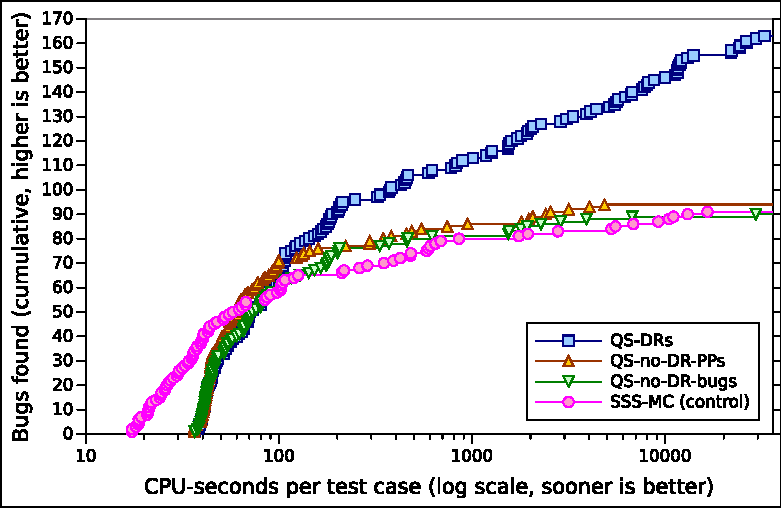
\includegraphics[width=0.48\textwidth]{dowefindbugsfaster-squashed.pdf} \\
		(a) Bugs found by elapsed CPU time. Overall, a more direct comparison than (b),
		although \quicksand's start-up overhead is exaggerated, as the SSS-MC tests are not parallelized. \\
		\\
	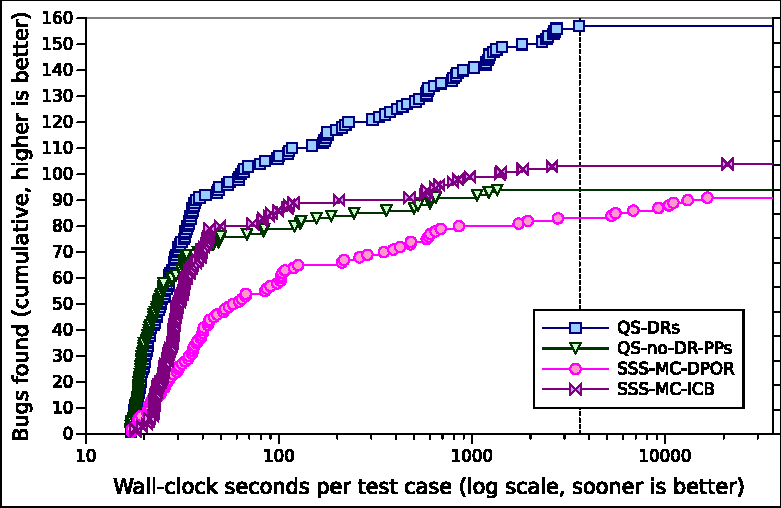
\includegraphics[width=0.48\textwidth]{dowefindbugsfaster-wallclock.pdf} \\
		(b) Bugs found by elapsed wall-clock time.
		\quicksand~is parallelized tenfold; the vertical line indicates its 1 hour limit. \\
	\end{tabular}
	}
	\caption{Comparison of bug-finding performance
	by several configurations of \quicksand~and the SSS-MC control.
	\quicksand~finds \revision{151}\% as many bugs with data-race PPs.}
	\label{fig:dowefindbugsfaster}
\end{figure}

{\bf Finding new data-race bugs.}
%We quickly pull ahead of SSS-MC, and ultimately conclude with 179\% as many bugs in total.
%The break-even point is at a negligible 90 seconds.
\revision{Compared to the best SSS-MC series, \quicksand~finds}~more bugs within any CPU budget greater than \revision{200}~seconds,
and ultimately concludes 10 CPU-hours with \revision{151}\% as many bugs in total.
\revision{Before the break-even point at 200 seconds,
% TODO
% (for SSS-MC-ICB) or XXX seconds (for SSS-MC-Shared-Mem)
\quicksand~lags behind the SSS-MC approaches due to additional start-up overhead from its tenfold parallelism.
However, converting SSS-MC's early CPU-time advantage into faster wall-clock performance remains an open research problem \cite{parallel-dpor}.
In Figure~\ref{fig:dowefindbugsfaster}(b), we give \quicksand~full credit for its inherent parallelism, and it outperforms SSS-MC for any fixed budget of wall-clock time.}

%{\bf Variance.}
% TODO CAMREADY: Probably will need at least a 3rd run of dis.
Because \quicksand~can be nondeterministic in its scheduling of state spaces,
we ran the QS-DR tests a second time to quantify the variance.
We found the area between the two QS-DR curves to be
% TODO
{\bf XX\%}
of the area between QS-DR and SSS-MC-ICB (the next closest),
% TODO cite
which we consider an insignificant amount of variance.
}


% TODO: Fix up this paragraph after preempt-everywhere results come in.
The left half of Table~\ref{tab:drbugs}
breaks down the number and types of bugs found by each test program.
In \mxtest, in which we do not trust the lock implementation's correctness,
the control experiment found dramatically fewer bugs (just 1)\footnote{
	The one bug SSS-MC found was in a fully-assembler lock implementation. {\tt yield()}'s return value clobbered a value stored in {\tt \%eax}, which could lead to a failure after two repeated contentions. Preempting only on {\tt yield()} (in the contention loop) was sufficient to find the bug.}.
%Intuitively, this is due to our control experiment being able to preempt only on the boundaries of the API which
%Though for many applications of MC, assuming a correct lock implementation is sufficient,
Though it often suffices to assume correctly-implemented locks,
we consider this strong evidence that new low-level synchronization code must be verified with data-race PPs.
%TODO CAMREADY: Run a mutex expt where "all atomic instrs" are PPs. See how many bugs are missed anyway.
% Wwe re-ran the \mxtest control experiment with \landslide~hard-coded to preempt on any atomic instruction
% (as well as on the mutex API boundaries).
% Still, this smarter configuration for SSS-MC found only 99999999999 bugs of \quicksand's 13.

%% RIP this.
%Furthermore, we plotted another line from this dataset, QS-no-DR-bugs,
%which represents only the bugs found in state spaces without any data-race PPs (like QS-no-DR-PPs, but paying any overhead for using data-race PPs).
%Intuitively, this line shows that for programs with only benign data races,
%\quicksand~can afford the extra overhead of verifying them while still slightly edging out SSS-MC.

% TODO: fix this table.
\begin{table*}[t]
	\begin{center}
		\small
	\begin{tabular}{r|c||c|c|c|c|c||c|c||c|c}
		% TODO: Update SSSMC column to have more favourable ICB numbers.
		& {\bf Num.} & {\bf DPOR} & {\bf QS} & {\bf DR-only} & {\bf Nondet.} & {\bf Malloc-} &
		{\bf Mutual} & {\bf Avg. tested} & {\bf Total} & {\bf Untested} \\
		{\bf Test name} & {\bf tested} & {\bf bugs} & {\bf bugs} & {\bf bugs} & {\bf DR bugs} & {\bf recycle DRs} &
		{\bf time-outs} & {\bf subset SSes} & {\bf DR PPs} & {\bf DR PPs} \\
		\hline
		% FIXME: update FRMs
				% #test  sssmc   qs      dronly  nondets  FRMs   timeout comp.SSes DRPPs untested DRPPs
		{\tt bcast}	& 79	& 7	& 11	& 4	& 4	& 51	& 0	& -	& 912	& 107	\\
		{\tt join} 	& 79	& 14 	& 24	& 10	& 6	& 333	& 5	& 60.8	& 781	& 292	\\
		{\tt mx} 	& 79	& 1	& 10	& 9	& 1	& 7	& 0	& -	& 829	& 1	\\
		{\tt sem} 	& 79	& 10	& 16	& 6	& 5	& 140	& 29	& 73.3	& 753	& 279	\\
		{\tt signal} 	& 79	& 4	& 10	& 7	& 6	& 180	& 10	& 54.2	& 1118	& 391	\\
		{\tt rwlock} 	& 79	& 26	& 28	& 2	& 2	& 125	& 19	& 29.6	& 915	& 634	\\
		\hline
		{\tt sched} 	& 59	& 1	& 7	& 6	& 4	& 0	& 0	& -	& 144	& 3	\\
		{\tt alarm} 	& 44	& 5	& 21	& 17	& 3	& 35 	& 22	& 9.1	& 115	& 89	\\
		{\tt wait} 	& 52	& 23	& 30	& 7	& 1	& 31	& 8	& 28.0	& 142	& 31	\\
		\hline
		{\bf Total}	& 629	& 91	& 157	& 68	& 32	& 902	& 93	& 42.6 	& 5709	& 1827	\\
	\end{tabular}
	\end{center}
	\caption{Summary of bugs and data races found by each test program.
		% TODO
		DPOR is the control; QS is \quicksand.
		``DR-only bugs'' counts among \quicksand's bugs how many required data-race PPs to expose (\sect{\ref{sec:eval-sssmc}});
	among those, ``Nondeterministic DR bugs'' counts how many candidates required MC integration to identify (\sect{\ref{sec:eval-dr}}).
	``Malloc-recycle DRs'' counts how many false positives we suppressed (\sect{\ref{sec:eval-dr}}).
	``Mutual time-outs'' counts how often both SSS-MC and \quicksand~timed out with no bug found;
	among those, ``Average tested subset SSes'' counts how many partial verifications \quicksand~provided on average for each test (\sect{\ref{sec:eval-sssmc}}).
	``Total DR PPs'' counts how many unique data-racing instructions we identified among tests where we found no bugs;
	among those, ``Untested DR PPs'' counts how many could not be checked in the time limit (\sect{\ref{sec:future}}).
		}
	\label{tab:drbugs}
\end{table*}

% TODO CAMREADY: Compare QS-ETAs to QS-Random to evaluate "smaller is better" claim.
{\bf Finding the same bugs faster.}
%To test whether Iterative Deepening is effective even for MC domains without data races, %such as message-passing distributed systems,
\revision{The QS-Sync-Only experiment tests whether}~Iterative Deepening is effective even for MC domains without data races.
\revision{When \quicksand~ignores all data-race candidates,
its results are competitive with SSS-MC-DPOR, but SSS-MC-ICB outperforms it.
This is unsurprising: the seed subsets of PPs (\sect{\ref{sec:initial-pp}}) QS-Sync-Only is limited to are much less flexible than ICB's preemption strategy.
This result suggests that in future work, \quicksand~should consider using ICB in parallel with its default configuration when it finds no data-race candidates to test.}
%\footnote{
%Because \quicksand~is not yet instrumented to subset hard-coded PPs beyond the 4 ways shown in Figure~\ref{fig:id},
%we ran these tests for 2.5 hours on 4 CPUs each.
%Future work could parallelize QS-no-DR-PPs further; see \sect{\ref{sec:future}}.}.

%Even though SSS-MC mostly catches up to it by the end of the 10-hour budget,
%and is faster in the first 60 seconds due to less start-up overhead,
%QS-no-DR-PPs finds more of the bugs sooner thereafter.
%Hence, for modest CPU budgets,
%\quicksand~is likely to find bugs SSS-MC will miss.
%and for more ambitiously-sized tests,
%programmers can be more confident in the verification provided when \quicksand~times out with no bug found.
%We conclude that for smaller arbitrary CPU budgets, especially less than 1 hour,
%Iterative Deepening is likely to find bugs SSS-MC will miss.
%Moreover, it is also easy to imagine scaling up the size of each test case to test ,
%using more threads or longer sequences of API calls.
%We hope that is compelling even to users willing to spend many CPU-hours on testing.
%These results show explicitly that for arbitrary CPU-time budgets
%\footnote{The initial perfect overlap between QS-DRs and QS-no-DR-bugs indicates how long it takes before the first data-race bug is found.}
%even after the extra overhead of verifying them, \quicksand~still slightly edges out SSS-MC

\revision{
On the other hand,
comparing QS-DR to SSS-MC-Shared-Mem shows that Iterative Deepening thoroughly outperforms ICB when shared-memory preemptions come into play.
%We attribute this to the fact that
Statically configuring a PP for every shared memory access in advance
produces orders of magnitude more PPs than
waiting for an access to be identified as part of a (potential) data race at runtime.
%
In principle, DPOR and BPOR should identify and prune any equivalences arising from extraneous PPs on non-conflicting accesses.
However, in practice,
%we found that
the sheer number of accesses during each new execution (often thousands) added significant performance overhead to the MC when computing DPOR and backtracking\footnote{
	\revision{The bug-finding performance of SSS-MC-ICB approach could be improved by heuristically
	%preempting only on data-race candidates found in advance by a single-pass analysis
	using a single-pass analysis to find data-race PP candidates in advance
	\cite{portend}, but this sacrifices soundness, as shown in \sect{\ref{sec:eval-dr}}.}
}.
Iterative Deepening avoids this overhead by waiting until runtime to identify fewer, more relevant PPs dynamically,
and is hence more suitable for MC with data-race PPs.}

{\bf Partial verification.}
When a MC job times out, the user may prefer a brief summary of what parts of the test were verified, rather than writing off all the CPU time as a waste.
%Beyond using the state space estimator to guess the percent coverage,
We know of no approach to quantify the probability
that a bug would be exposed by an untested interleaving,
but \quicksand~at least reports which subsets of PPs resulted in state spaces that did complete in time.
%\quicksand~does not attempt any such quantitative guarantee,
%but can at least report
On 129 tests, the SSS-MC control experiment timed out after 10 hours with no bugs found.
Among these tests, \quicksand~found bugs in 36.
For the other 93, we show the number of state spaces \quicksand~was able to complete in the ``Average tested subset SSes'' column of Table~\ref{tab:drbugs}.
%and the number of unique PPs among them.
%In 6 cases, \quicksand~also failed to complete anything; beyond these,
%between 1 and 253 state spaces were completed for each test
%Between 0 and 233 unique PPs were tested among some completed subsets, with a mean of 27.2 and median of 7.5.
These completions guarantee that, if the test program could expose a bug,
% Justify implicit hypothesis: Sync PPs + DR PPs = all possible relevant PPs.
it would only be found by a new data-race PP not discovered yet, or by a superset combination of PPs not reached.

%Hence, in Table~\ref{tab:drbugs} we count how often \quicksand~uncovered a bug only in state spaces which included data-race PPs, while
%
%In Table~\ref{tab:allbugs} ....

{\bf Full verification.}
% TODO: Discuss how ICB sucks even more.
For 153 of our 629 tests, \quicksand~was able to provide the total verification guarantee described in \sect{\ref{sec:totalverif}}.
In Figure~\ref{fig:totalverif} we plot the cumulative distribution of \quicksand's total verifications
%before a given elapsed CPU consumption.
\revision{against those provided by SSS-MC-Shared-Mem\footnote{
	\revision{In kernel or thread library code, a thread's own stack accesses may not always be private. %assumption may not hold.
	For example, many P2 condvars use stack-allocated list nodes to track waiting threads.
	SSS-MC-Shared-Mem's verifications are only sound in the absence of such sharing!
	\quicksand~detects these dynamically, without needing to discriminate between stack and heap.}
	%Expanding the statically-coded PPs to include stack accesses would make SSS-MC-Shared-Mem's performance even worse.
	% Especially for testing kernel-level code, deciding which of a thread's memory accesses are shared versus private is nonstraightforward, as threads may share data structures allocated on their own stacks for synchronization. Hence, the common heuristic of ignoring stack accesses as private (which we employ for this control experiment) introduces some unsoundndess.
}.
\quicksand~outperforms SSS-MC, being able to verify safety for
% TODO
{\bf 99x}
as many tests in 10 CPU-hours.
We attribute this again to the overhead of the sheer number of statically-coded PPs that SSS-MC-Shared-Mem must use,
as well as to the work which ICB necessarily repeats when increasing its preemption bound.}

Among these verified tests, 36 contained no data-race candidates whatsoever,
so the same verification could be provided
%by SSS-MC
\revision{with synchronization PPs only.
We plot the verifications by QS-Sync-Only, SSS-MC-DPOR and SSS-MC-ICB as well:
among these, the otherwise more antiquated SSS-MC-DPOR performs best,
while the other two lag behind
}
%\quicksand~is slower than SSS-MC-DPOR
due to redundant work (\sect{\ref{sec:future}}).
\revision{While QS-Sync-Only and SSS-MC-ICB are competitive with each other},
using data-race PPs increases our \revision{verification capacity}~by 4.25x.

\begin{figure}[t]
	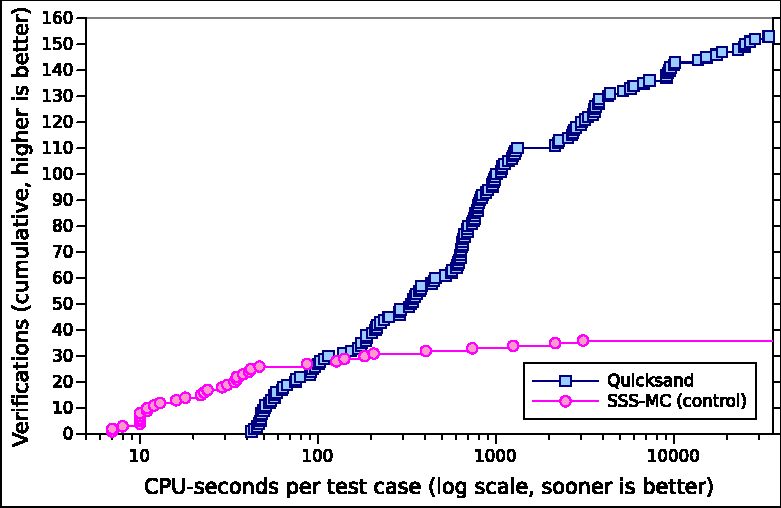
\includegraphics[width=0.48\textwidth]{totalverifs-squashed.pdf}
	\caption{Cumulative distribution of tests \quicksand~fully verified (\sect{\ref{sec:totalverif}}).
	Some tests had no data-race candidates, and hence could also be verified by SSS-MC.}
	\label{fig:totalverif}
\end{figure}


%%%%%%%%%%%%%%%%%%%%%%%%%%%%%%%%%%%%%%%%%%%%%%%%%%%%%%%%%%%%%%%%%%%%%%%%%%%%%%%%

\subsection{Comparing to single-pass data-race analysis}
\label{sec:eval-dr}
% Though we mechanically verify whether each data race candidate leads to a bug, each new PP can increase combinatorially..... obviously wish to avoid...

Beyond finding new bugs with data-race PPs, we evaluated \quicksand's performance for classifying data-race candidates in two ways.

{\bf Suppressing ``malloc-recycle'' false positives.}
In \sect{\ref{sec:recycle}} we showed the soundness of suppressing data race reports between two heap accesses when the surrounding memory was re-allocated in between.
In Table~\ref{tab:drbugs}, the column ``Malloc-recycle DRs'' shows the total number of such data-race candidates for each test program.
In total, 902 data-races fit the malloc-recycle pattern across all tests,
only 69 of which were observed to avoid the re-allocation in an alternate interleaving.
Our proof in \sect{\ref{sec:recycle}} guarantees the safety of pruning all 833 other state spaces.

Among those 69 true data-races, %which initially fit the malloc-recycle pattern,
none exposed a new bug when used as a PP.
This suggests that for other data-race tools,
suppressing malloc-recycle candidates may be a productive heuristic,
even if unsound without Iterative Deepening.
However, \quicksand~was able to correctly identify the 69 violations of that heuristic (among 30 distinct tests),
and fall back to classifying them with DPOR.
%which we consider a much stronger verification.

%%%%%%%%%%%%%%%%%%%%%%%%%%%%%%%%%%%%%%%%%%%%%%%%%%%%%%%%%%%%%%%%%%%%%%%%%%%%%%%%

%For the [NONDET] expt, you don't need to additionally count how many DRs
%needed to be found in a DR-PP state space, because when EXPLORE_BACKWARDS=0,
%you'll need to preempt on the DR PP to find the new DR anyway, hence they will
%be nondet. Unless you want to separately count the subset of nondet drs that
%are also dr-pp-ss-only (the reviewers may ask for this before cam-ready?).
{\bf \revision{Finding nondeterministic data-race candidates}.}
Some memory accesses may be hidden in a control flow path that requires a nondeterministic preemption to be executed.
In such cases, a single-pass dynamic data-race detector
%could not achieve the coverage necessary
could fail
to identify a racing access pair as a candidate to begin with.
%
We counted how many such data-races, used as PPs, led to \quicksand~finding new bugs,
thereby making them {\em false negatives} of the single-pass approach.
We classified each data-race candidate according to whether \landslide~reported them during the first interleaving,
before any backtracking or preempting:
if so, they were {\em single-pass data races}; otherwise, {\em nondeterministic}.

To ensure a fair comparison, we disabled \landslide's {\em false-positive}-avoidance techniques during this experiment.
For example, we reported malloc-recycle data races during the first interleaving, as a single-pass analysis must
%rather than waiting until future interleavings to witness them without the malloc-recycle pattern
(\sect{\ref{sec:recycle}}).
This prevents \landslide~from suppressing an observed data race on the first interleaving,
which would falsely classify it as nondeterministic.

\begin{figure}[t]
	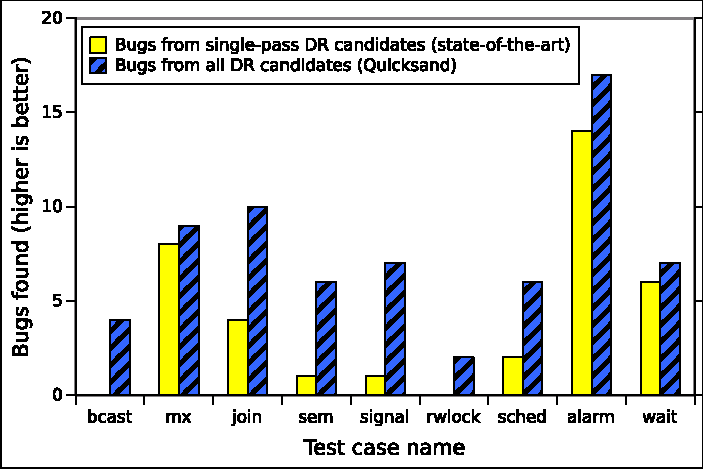
\includegraphics[width=0.48\textwidth]{nondet-drs-1-v2.pdf}
	\caption{Some data-race candidates may not be identified during a single program execution.
		Using nondeterministic data races as PPs,
		\quicksand~found 189\% as many data-race bugs compared to using single-pass candidates alone.
	}
	\label{fig:dr-falsenegs}
\end{figure}
Figure~\ref{fig:dr-falsenegs} compares the types of data-race candidates necessary to expose each data-race bug in our test suite.
The first series represents the bugs found using PPs from single-pass data-race candidates,
% not entirely true, as portend could be given data-race traces from an MC,
%but they don't do it in their paper, so i feel comfortable making this claim
i.e., the state-of-the-art approach used by \cite{racefuzzer,portend}.
The second series shows all data-race bugs \quicksand~found,
which includes the former type as well as new bugs involving nondeterministic data-races.
\quicksand~found 68 data-race bugs in total, only 36 of which could be found with single-pass data-race candidates alone.
%In total, we found 189\% as many bugs by using nondeterministic data-race candidates as PPs.

%When proving that [NONDET] dr buges exist, make sure to mention that, although
%their frequency varies depending on test case (mx test: almost none; bct:
%almost all), they are still PRESENT in all (or almost all) test cases, meaning
%it is not just a matter of writing better test cases.

Note that we are not comparing how much testing time is required before identifying the data-race candidates involved in each bug.
Single-pass data races can all be found after a single program execution,
while \quicksand~may potentially take up to all 10 CPU-hours before identifying a nondeterministic data race.
However, prior work data-race tools \cite{tsan}, being not integrated with a MC,
are not intended to discover new candidates under subsequent runs.
Running a single-pass data-race tool repeatedly for 10 CPU-hours could potentially uncover some nondeterministic candidates,
but stress testing's comparative problem with achieving reliable coverage is already well-understood
\cite{chess-icb,gambit}.
Likewise, replay-based tools \cite{portend} are dependent upon the data-race detector to provide an execution trace leading to each candidate.
This experiment suggests that
such tools could benefit from a similar feedback loop as used in Iterative Deepening.
%i.e., discovering transitively-reachable data races while testing initial ones.
%although that would still not simultaneously be able to provide total verifications.
% TODO: read gambit paper


% Figure out concretely what the data race tricks are that we do, so we can claim them as contributions in the paper. Then ACTUALLY EVALUATE THEM.
%         - Speculative DR PPs.
%                 Not a heuristic, rather how to make it work at all to begin with.
%                 (Cite MS thesis, claim on backwards explorating finding bugs faster)
%         - Free/re-malloc to eliminate some false positives. See #193.
%                 Measure how many false positives are eliminated.
%                 Check, ofc, to make ABSOLUTE SURE, that no bugs missed w/ this trick.
%                         If there are, it could be because of the implementation
%                         bug described in #193.
%         - Using tid/last_call filtering because whole stack traces are too expensive.
%                 Moderately optional, 1st priority since theoretically interesting:
%                 Turn on/off and measure how resulting DR bug #s change.
%         - Optional: Reprioritizing DRs based on "confirmed" / "suspected"
%                 Shouldn't be hard just make ID wrapper print "s" or "c"!
%                 Is it helpful for ID to put priorities on DR PPs?
%                         Test by inverting the priority and see if fewer buges are found.
%         // Super optional to talk about. Probably not worth the time.
%         // - "Too suspicious" (during init/destroy)
%         //      (Cite eraser, section 2.2)

\section{Discussion}
\label{sec:future}

In this section, we discuss \quicksand's limitations and opportunities for future improvement.

% TODO CAMREADY: Measure how much subset overlap there is.
{\bf Avoiding redundant work.}
When we extend a small state space with more PPs, the new state space is guaranteed to test a superset of interleavings compared to the old one.
Any interleaving which does not preempt threads on any of the new PPs will be repeated work.
%Because we prioritize completing small state spaces before extending them with more PPs,
%the superset state spaces we run later will repeat each branch of their already-completed subsets.
%
%We measured the proportion of repeated work among completed state spaces across our test suite;
%on average, {\bf \large 999\%} of the interleavings in each test were repeated, with some tests as high as {\bf \large 9999\%}.
This may make us slower than SSS-MC to find certain bugs,
for example, if both {\tt lock} and {\tt unlock} PPs together expose a bug, but not either alone.
%Similarly, when pursuing total verification (\sect{\ref{sec:totalverif}}),
%if the state space resulting from preempting on every instruction could be completed,
%an SSS-MC tool such as \cite{spin} might achieve that verification faster,
%as Iterative Deepening will test many subsets of data-race PPs first.
Predicting whether an upcoming interleaving has already been tested is not straightforward,
but we believe future implementations
%of Iterative Deepening
could incorporate cross-job memoization
to prune some or all such repeated work.

{\bf Finer-grained PP subsets.}
\quicksand~was able to partially guarantee safety for some PPs in 89\% of tests with too-large maximal state spaces.
However, in 4 cases, no more than the minimal state space could be verified,
and in 6 others, no state spaces were completed at all.
%Larger state spaces often result from finer-grained locking,
%which can indicate a more intricate concurrent algorithm or an unnecessarily complicated design.
%Such programs may require even more rigorous verification than a program with a single global lock.
%Hence these corner cases are important to consider for future work.
While we used {\tt within\_function} (\sect{\ref{sec:landslide}}) {\em statically} to restrict where PPs could arise in advance of the test,
%we envision
future
%Iterative Deepening
implementations could use this mechanism to {\em dynamically} subset PPs further,
making partial verification of larger tests possible.
%enabling partial verification of such large tests. % if need space
%Because our current implementation does not avoid repeated interleavings across state spaces,
%as discussed above,
%we were limited to a small number of very basic PP subsets to statically seed the exploration

%{\bf Small test cases.}

{\bf Partial verification.}
%We are not the first to provide a partial verification guarantee when timing out on too-large state spaces (\sect{\ref{sec:eval-sssmc}}).
While we guarantee safety when using certain combinations of PPs (\sect{\ref{sec:eval-sssmc}}),
Iterative Context Bounding
guarantees safety under no more than a certain number of preemptions \cite{chess-icb}.
%according to the maximum bound reached in the time limit.
%We imagine
These guarantees could each be useful to developers in different scenarios,
and future work could combine the two approaches to provide both at once.
One benefit of our technique is that {\tt within\_function} %-based Iterative Deepening (discussed above)
would enable expert developers to
%configure custom subsets of PPs they are most interested in verifying,
%according to which modules of a codebase they wish to test.
restrict Iterative Deepening to only the modules of a codebase they wish to test.

Likewise, when full verification is not computationally feasible,
some jobs with data-race PPs will time out.
We cannot guarantee those races are
%false positives or
benign, even though no bug was found.
In the ``Untested DR PPs'' column of Table~\ref{tab:drbugs}, we show how many such candidates we could not verify (32\%).
For a more formal treatment of these cases, we refer the reader to the {\em k-witness harmless} metric introduced by \cite{portend},
which could be combined with \quicksand~in future work.
% Future work: Add parallel DPOR so you can fill your spare CPUs when there are fewer than the max number of jobs.

\section{Related Work}
\label{sec:related}

\subsection{Stateless Model Checking}

We build upon many established model-checking techniques, dating back
% of course
to Verisoft, the original C model checker \cite{verisoft}.
%, and Eraser, the original data race detector \cite{eraser}.
%Our model checker
%\landslide~\cite{landslide} itself implements many techniques from prior work (\sect{\ref{sec:landslide}}).
%itself implements DPOR \cite{dpor},
%state space estimation \cite{estimation},
%and data-race detection \cite{eraser}.
We compare related tools by their treatment of shared-memory thread communication.

{\bf Synchronization events only.} CHESS \cite{chess} and dBug \cite{dbug-ssv} instrument the thread library API, and can preempt programs only during calls to this API.
Hence, they will miss any bugs that require interleaving threads at instruction granularity during a data race. CHESS provides a data-race analysis to report any such violations of its concurrency model to the user, but does not incorporate data-race candidates as PPs in future tests.

{\bf Message-passing.} Other stateless model checkers, such as SAMC \cite{samc}, MaceMC \cite{macemc}, MoDist \cite{modist}, ETA \cite{dbug-retreat}, and Concuerror \cite{optimal-dpor},
limit thread communication to a message-passing API to more effectively test distributed systems.
This eliminates the need for data-race analysis, but restricts the class of programs that can be tested.
Nevertheless, Iterative Deepening is applicable to these tools.

{\bf Preempting at instruction granularity} is a prerequisite for using data-race PPs.
However, the resulting state space explosion demands that any such tool either
choose a small subset of instructions to consider as PPs
or be limited to very small test programs.
%However, every such prior tool we know of has serious drawbacks.
SKI \cite{ski} approaches kernel code by statically choosing a random set of instructions in advance, %offsets from the start of the test,
which is perhaps more similar to
%stress testing or
schedule fuzzing \cite{randomized-scheduler} than to exhaustive state space exploration.
%
SPIN \cite{spin} specializes in verifying synchronization primitive implementations such as RCU \cite{rcu}, which is similar to our \mxtest~experiment,
although it requires code to be written in the PROMELA language.
%However, SPIN is stateful rather than stateless, and explicitly storing visited program states rather than using DPOR limits the size of programs that can be practically tested.
%
Inspect \cite{inspect} instruments source code by inserting wrapper calls around all accesses to potentially-shared data.
It identifies such instructions in advance with an over-approximating alias analysis,
while \landslide~\cite{landslide} traces the memory locations of accesses at runtime.
Both SPIN and Inspect fix their set of PPs in advance, so could be
%combined with \quicksand~
extended with Iterative Deepening in future work.
%so cannot check implementations directly.

{\bf Other techniques.} Various improvements or alternatives to DPOR have been developed, such as Dynamic Interface Reduction \cite{demeter}, Maximal Causality Reduction \cite{mcr},
%DPOR for relaxed memory models \cite{tsopso},
and SAT-directed MC \cite{satcheck}.
These are all compatible with our technique.
Recent work \cite{tsopso} has extended DPOR for relaxed memory models \cite{memory-consistency-models},
which we do not yet account for in our proofs (\sect{\ref{sec:soundness}}).
Parrot \cite{parrot} combines MC with a partially-determinizing runtime for further reduction, but still, fewer than half the non-trivial state spaces in their evaluation could be completed.
%providing a strong argument for \quicksand.
Finally, Iterative Context Bounding (ICB) \cite{chess-icb} is most similar to our work,
as both approaches provide a partial verification
%on some subset of interleavings
when full completion is intractable (\sect{\ref{sec:future}}).
However, ICB is limited to a fixed set of PPs, and to our knowledge no algorithm has been proposed to dynamically add data-race PPs during a test with ICB.

\subsection{Data Race Detection}
\label{sec:related-dr}

%Too many related projects to list have made contributions to the
Many advances have been made on the false-positive data race problem since it was first introduced in \cite{eraser}.
\cite{hybriddatarace} and \cite{tsan} combine the lockset and happens-before analyses into a hybrid technique, which we employ.
DroidRacer \cite{droidracer} and CAFA \cite{cafa} target
%event-driven
Android applications, using domain-specific heuristics (orthogonal to our method) to reduce false positives. % cut for space?
Like \landslide, DataCollider \cite{datacollider} offers data-race techniques for kernel code.
IFRit \cite{ifrit}
improves performance using an interference analysis,
which would allow future work to avoid tracing every memory access.
%although in our context, we cannot admit false negatives (\sect{\ref{sec:totalverif}}).
% No, IDGAF about pure happens before.
%FastTrack \cite{fasttrack} optimizes the performance of pure happens-

Closer to our work, replay analysis \cite{recordreplaydrs} also suppresses false positives by testing multiple thread interleavings.
%after finding data race candidates.
This work compares the immediately resulting program states for differences,
preferring to err on the side of false positives.
RaceFuzzer \cite{racefuzzer} avoids false positives by requiring an actual failure be exhibited, as we do,
although it uses random schedule fuzzing rather than stateless MC.
While this technique can also classify malloc-recycle candidates as false positives (\sect{\ref{sec:recycle}}),
they require replaying the threads in a new interleaving.
Moreover, \cite{portend} argues that accurate classification may require many re-executions,
%according to many pre- and post-race sequences,
which is tantamount to adding a new state space in \quicksand.
Our proof in \sect{\ref{sec:recycle}} allows us to eliminate this special case with no additional replay beyond what DPOR already requires.

Portend \cite{portend} is the most closely related work we have found.
Based on single-pass data race reports, it tests alternate program executions to classify candidates in a taxonomy of likely severity.
It uses symbolic execution to test input nondeterminism as well as schedule nondeterminism,
%while we explore the latter only.
and additionally reports non-failing races which nevertheless cause
%suspiciously
different program output. %, which is orthogonal to our technique.
However, Portend does not test alternate interleavings {\em in advance} of knowing any specific data races,
which is necessary to expose certain bugs (\sect{\ref{sec:eval-falseneg}}) or to provide full verification (\sect{\ref{sec:totalverif}}).
% Not really true.
%It also assumes the POSIX synchronization API, so cannot verify arbitrary synchronization algorithms such as we do with \mxtest.
Future work could combine the two approaches, using MC to produce new data-race traces for Portend to classify, or using Portend's analysis to inform \quicksand's heuristic priorities.

% \subsection{Other Concurrency Testing Approaches}
%
% blah blah pldi'15 symbiosis DSP

% Note that BPOR paper claims that ICB(3+) repeats LOADS of work, and that makes it ok for landslide-ID to repeat work.

% IDK if i should mention it, but OOPSLA 2015, protocol based verification of MPI concurrency paper. Different verification approach entirely; doesn't suffer exponential explosion but limited to programs with no shared state and MPI communication only

% Probably NOT worth a mention: OOPSLA 2015, stateless model checking of event driven applications. Turning timer-driven model on its head and checking single-threaded, but asynch-event-driven programs (i.e. device-like signal handlers)


%%%%%%%%%%%%%%%%%%%%%%%%%%%%%%%%%%%%%%%%%%%%%%%%%%%%%%%%%%%%%%%%%%%%%%%%%%%%%%%%

\section{Conclusion}
\label{sec:conclusion}

%We are great. Accept our paper.

We have presented Iterative Deepening and \quicksand, a new technique and tool for automating the choice of preemption points (PPs) during stateless model checking.
% , and \quicksand, a tool which implements this technique tailored to the \landslide~model checker.
\quicksand~incorporates data-race analysis to create new PPs tailored specifically to the program under test,
and manages multiple model checker instances to test many different PP subsets in a given CPU budget, even when the full state space of all PPs would be computationally intractable.

Our evaluation shows that \quicksand~achieves better bug-finding results than either single-pass data-race detection or single-state-space model checking alone.
%We dramatically reduce false-positive data race reports,
%%by verifying the absence of bugs in their associated state spaces
%and find bugs caused by nondeterministic data-races in alternate thread interleavings missed entirely by single-pass analysis.
%Compared to prior work,
%, we find bugs faster in smaller subset state spaces, %% not true, or at least, not by very much
%when the maximal state space is too large to explore
We find new bugs with data-race PPs that could not be exposed by preempting only on synchronization APIs.
Moreover, when all data-race PPs can be fully tested within the CPU budget, we provide a verification as strong as if every single instruction had been used as a PP.

%Although \landslide~itself is not publicly available due to its dependency on the non-free simulator \simics, \quicksand~is open-source and its interface can be adapted to fit any similar tool.
\quicksand~is open-source and its interface can be adapted to fit any tool similar to \landslide.
We have also posted our evaluation's full data set. %and logs.
They are available at:

% TODO CAMREADY: Make data set, at least, public.

{\em github links removed for double-blind review}
%\url{https://github.com/bblum/landslide} % POST-SUBMISSION TODO: put QS in its own repository
%
%\url{https://github.com/bblum/landslide} % POST-SUBMISSION TODO: put final logs somewhere
% TODO CAMREADY: Don't forget to anonymize the names of all your grupos.

%\section{Acknowledgements}

% TODO CAMREADY
%{\em removed for double-blind review}
%Many thanks to Vaishaal Shankar, Haryadi Gunawi, and David A. Eckhardt for generously providing student implementations from Berkeley's, U. of chicago's, and CMU's OS classes respectively.
%Thanks to Wind River for the use of their simulator \simics.
%Thanks to
%Ji\v{r}\'{i} \v{S}im\v{s}a, Joshua Wise, Jean Yang, Brandon Lucia, Haryadi Gunawi, John Wilkes, and
%the anonymous PLDI reviewers for their helpful comments.
%This work was supported in part by
%the U.S. Army Research Office under grant number W911NF0910273.


\bibliographystyle{abbrvnat}
\bibliography{citations}{}

\end{document}
